\hypertarget{plotting}{%
\chapter{Plotting}\label{plotting}}

This chapter presents ways to create figures and graphs, more generally
called \textbf{data visualizations}. As examples, we'll generate three
figures:

\begin{itemize}
\item
  We'll replicate a figure from the Pew Research Center that shows
  changes in religious affiliation in the U.S. over time.
\item
  We'll replicate the figure from \emph{The Economist} that shows the
  prices of sandwiches in Boston and London (we saw this data back in
  Chapter 3).
\item
  We'll make a plot to test Zipf's law, which describes the relationship
  between word frequencies and their ranks.
\end{itemize}

With the tools in this chapter, you can generate a variety of simple
graphs. We will see more visualization tools in later chapters.

But before we get started with plotting, we need a new language feature:
keyword arguments.

\hypertarget{keyword-arguments}{%
\section{Keyword arguments}\label{keyword-arguments}}

When you call most functions, you have to provide values. For example,
when you call \passthrough{\lstinline!np.exp!}, the value you provide is
a number:

\begin{lstlisting}[]
import numpy as np

np.exp(1)
(@\dashfill@)
@@@2.718281828459045@@@
\end{lstlisting}

When you call \passthrough{\lstinline!np.power!}, you have to provide
two numbers:

\begin{lstlisting}[]
np.power(10, 6)
(@\dashfill@)
@@@1000000@@@
\end{lstlisting}

The values you provide are called \textbf{arguments}. Specifically, the
values in these examples are \textbf{positional arguments} because their
position determines how they are used. In the second example,
\passthrough{\lstinline!power!} computes \passthrough{\lstinline!10!} to
the sixth power, not \passthrough{\lstinline!6!} to the 10th power
because of the order of the arguments.

Many functions also take \textbf{keyword arguments}, which are optional.
For example, we have previously used \passthrough{\lstinline!int!} to
convert a string to an integer.

\begin{lstlisting}[]
int('21')
(@\dashfill@)
@@@21@@@
\end{lstlisting}

By default, \passthrough{\lstinline!int!} assumes that the number is in
base 10. But you can provide a keyword argument that specifies a
different base. For example, the string \passthrough{\lstinline!'21'!},
interpreted in base 8, represents the number
\passthrough{\lstinline!2 * 8 + 1 = 17!}. Here's how we do this
conversion using \passthrough{\lstinline!int!}.

\begin{lstlisting}[]
int('21', base=8)
(@\dashfill@)
@@@17@@@
\end{lstlisting}

The string \passthrough{\lstinline!'21'!} is a positional argument. The
integer value \passthrough{\lstinline!8!} is a keyword argument, with
the keyword \passthrough{\lstinline!base!}.

Specifying a keyword argument looks like an assignment statement, but it
does not create a new variable. And when you specify a keyword argument,
you don't choose the variable name. In this example, the keyword name,
\passthrough{\lstinline!base!}, is part of the definition of
\passthrough{\lstinline!int!}. If you specify another keyword name, you
get an error.

\textbf{Exercise:} The \passthrough{\lstinline!print!} function takes a
keyword argument called \passthrough{\lstinline!end!} that specifies the
character it prints at the end of the line. By default,
\passthrough{\lstinline!end!} is the newline character,
\passthrough{\lstinline!\\n!}. So if you call
\passthrough{\lstinline!print!} more than once, the results normally
appear on separate lines, like this:

\begin{lstlisting}[]
for x in [1, 2, 3]:
    print(x)
(@\dashfill@)
@@@1
2
3@@@
\end{lstlisting}

Modify the previous example so it prints the elements of the list, all
on one line, with spaces between them. Then modify it to print an open
bracket at the beginning and a close bracket and newline at the end.

\hypertarget{religious-affiliation}{%
\section{Religious affiliation}\label{religious-affiliation}}

Now we're ready to make some graphs.

In October 2019 the Pew Research Center published ``In U.S., Decline of
Christianity Continues at Rapid Pace'' at
\url{https://www.pewforum.org/2019/10/17/in-u-s-decline-of-christianity-continues-at-rapid-pace}.
It includes this figure, which shows changes in religious affiliation
among adults in the U.S. over the previous 10 years.

As an exercise, we'll replicate this figure. It shows results from two
sources, Religious Landscape Studies and Pew Research Political Surveys.
The political surveys provide data from more years, so we'll focus on
that.

The data from the figure are available from Pew Research at
\url{https://www.pewforum.org/wp-content/uploads/sites/7/2019/10/Detailed-Tables-v1-FOR-WEB.pdf},
but they are in a PDF document. It is sometimes possible to extract data
from PDF documents, but for now we'll enter the data by hand.

\begin{lstlisting}[]
year = [2009, 2010, 2011, 2012, 2013, 2014, 2015, 2016, 2017, 2018]
\end{lstlisting}

\begin{lstlisting}[]
christian = [77, 76, 75, 73, 73, 71, 69, 68, 67, 65]
\end{lstlisting}

\begin{lstlisting}[]
unaffiliated = [17, 17, 19, 19, 20, 21, 24, 23, 25, 26]
\end{lstlisting}

The library we'll use for plotting is Matplotlib; more specifically,
we'll use a part of it called Pyplot, which we'll import with the
nickname \passthrough{\lstinline!plt!}.

\begin{lstlisting}[]
import matplotlib.pyplot as plt
\end{lstlisting}

Pyplot provides a function called \passthrough{\lstinline!plot!} that
makes a line plot. It takes two sequences as arguments, the
\passthrough{\lstinline!x!} values and the \passthrough{\lstinline!y!}
values. The sequences can be tuples, lists, or arrays.

\begin{lstlisting}[]
plt.plot(year, christian);
\end{lstlisting}

\begin{center}
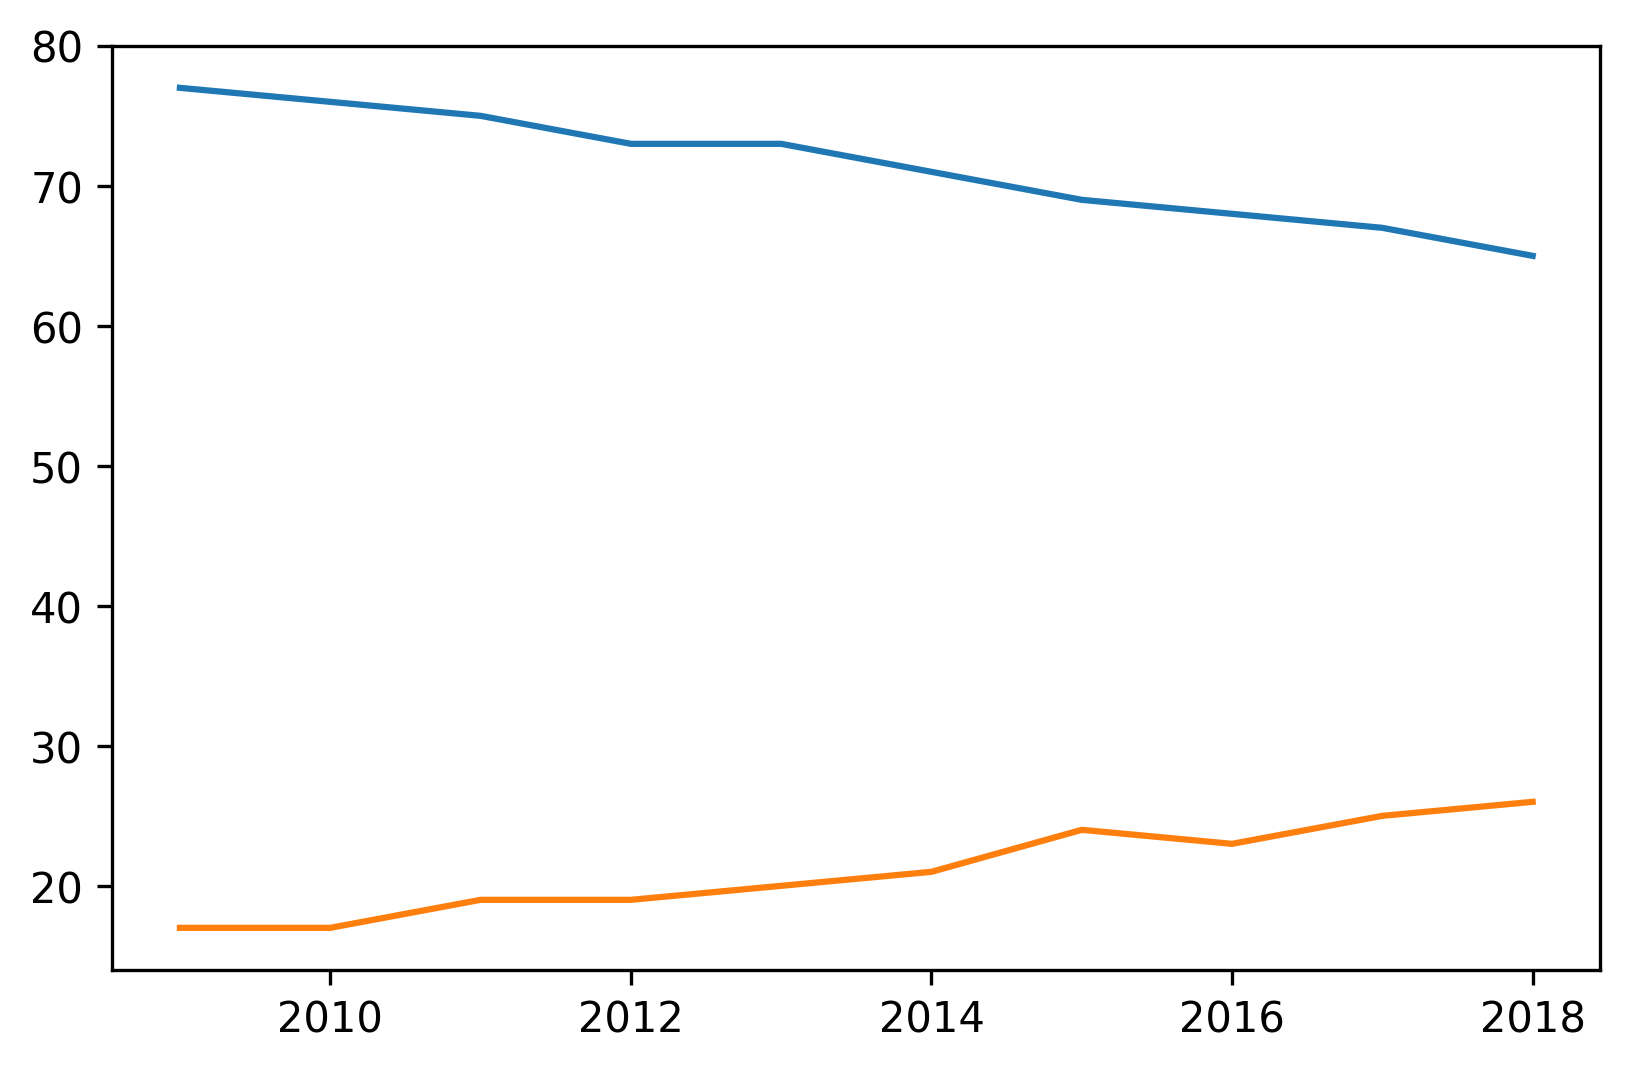
\includegraphics[width=4in]{chapters/06_plotting_files/06_plotting_24_0.png}
\end{center}

The semi-colon at the end of the line cleans up the output; without it,
the return value from \passthrough{\lstinline!plot!} would be displayed
above the figure.

If you plot multiple lines in a single cell, they appear on the same
axes.

\begin{lstlisting}[]
plt.plot(year, christian)
plt.plot(year, unaffiliated);
\end{lstlisting}

\begin{center}
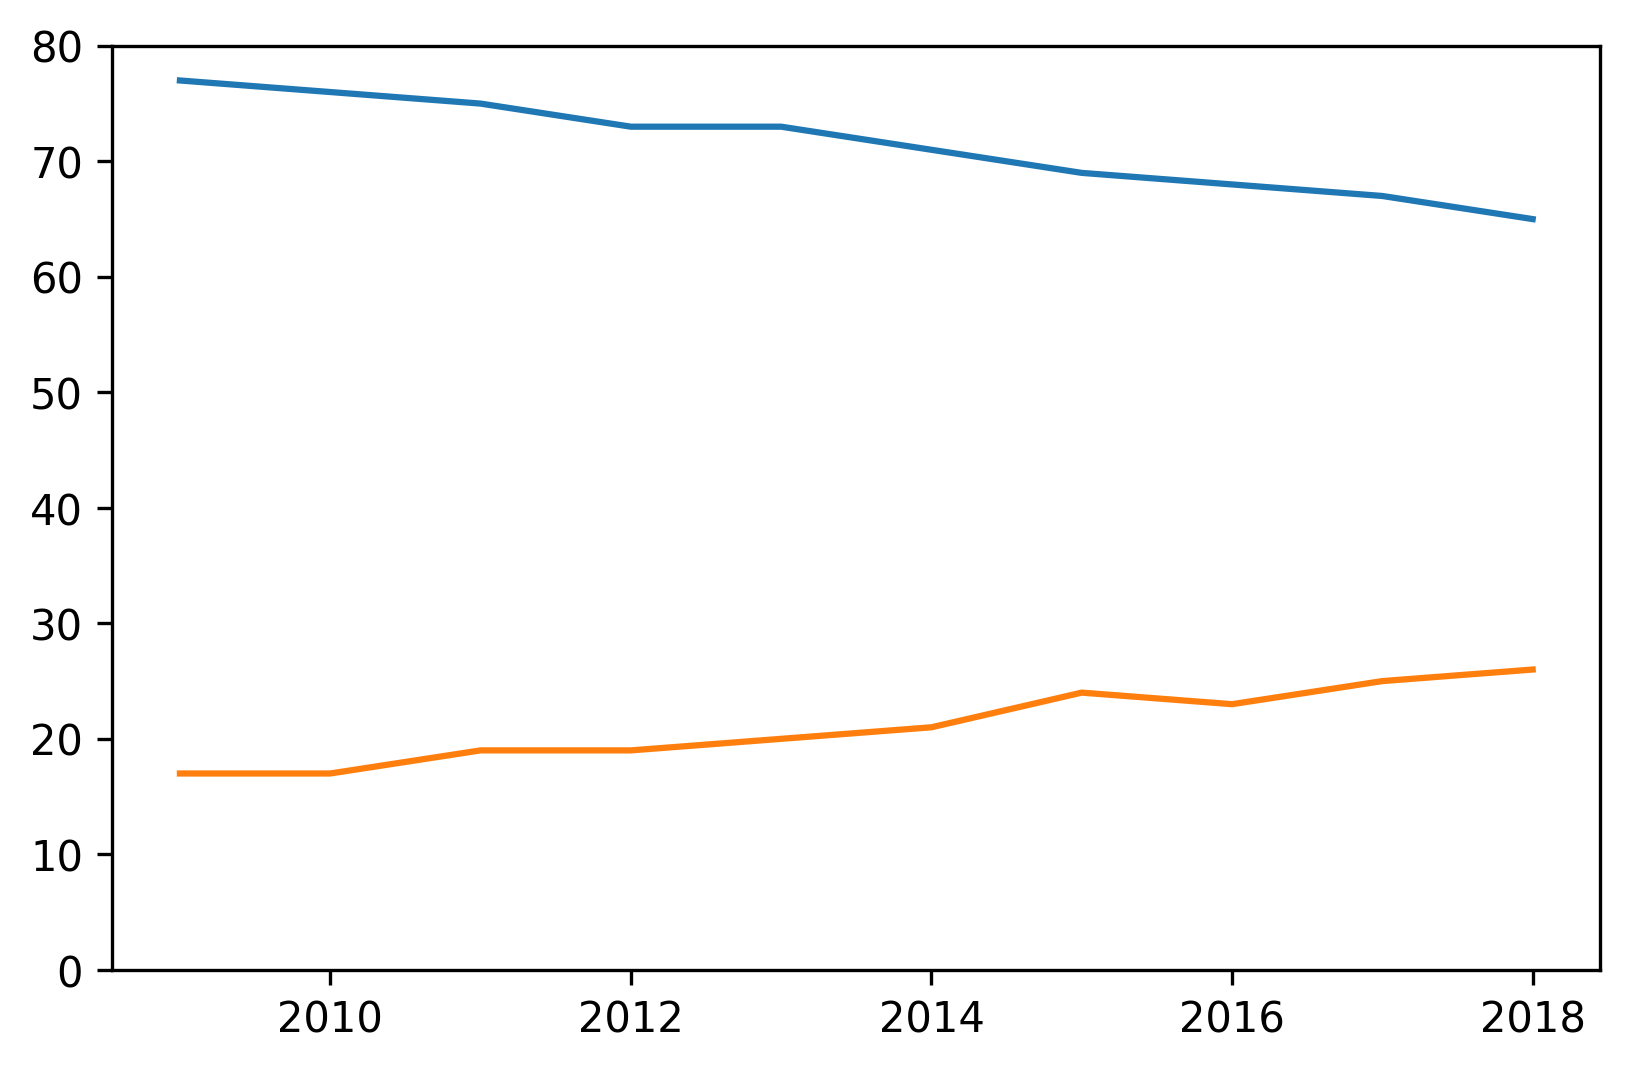
\includegraphics[width=4in]{chapters/06_plotting_files/06_plotting_26_0.png}
\end{center}

Plotting them on the same axes makes it possible to compare them
directly. However, notice that Pyplot chooses the range for the axes
automatically; in this example the \passthrough{\lstinline!y!} axis
starts around 15, not zero.

As a result, it provides a misleading picture, making the ratio of the
two lines look bigger than it really is. We can set the limits of the
\passthrough{\lstinline!y!} axis using the function
\passthrough{\lstinline!plt.ylim!}. The argument is a list with two
values, the lower bound and the upper bound.

\begin{lstlisting}[]
plt.plot(year, christian)
plt.plot(year, unaffiliated)

plt.ylim([0, 80]);
\end{lstlisting}

\begin{center}
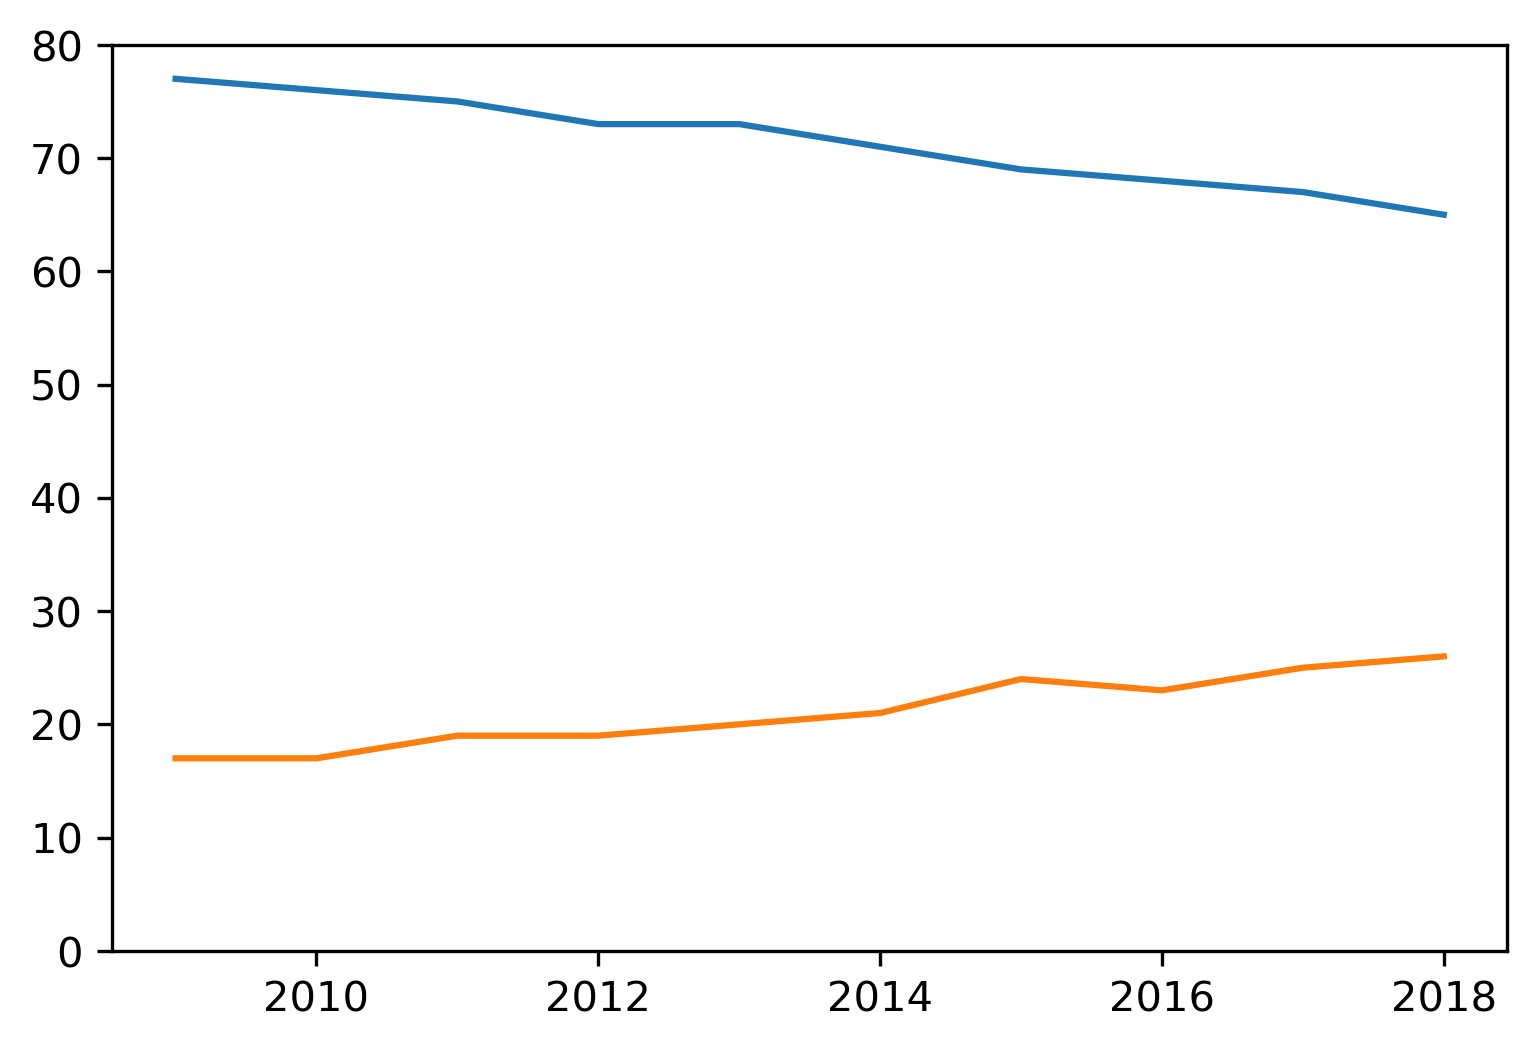
\includegraphics[width=4in]{chapters/06_plotting_files/06_plotting_28_0.png}
\end{center}

That's better, but this graph is missing some of the most important
elements: labels for the axes and a title.

\hypertarget{decorating-the-axes}{%
\section{Decorating the Axes}\label{decorating-the-axes}}

To label the axes and add a title, we'll use Pyplot functions
\passthrough{\lstinline!xlabel!}, \passthrough{\lstinline!ylabel!}, and
\passthrough{\lstinline!title!}. All of them take strings as arguments.

\begin{lstlisting}[]
plt.plot(year, christian)
plt.plot(year, unaffiliated)

plt.ylim([0, 80])
plt.xlabel('Year')
plt.ylabel('% of adults')
plt.title('Religious affiliation of U.S adults');
\end{lstlisting}

\begin{center}
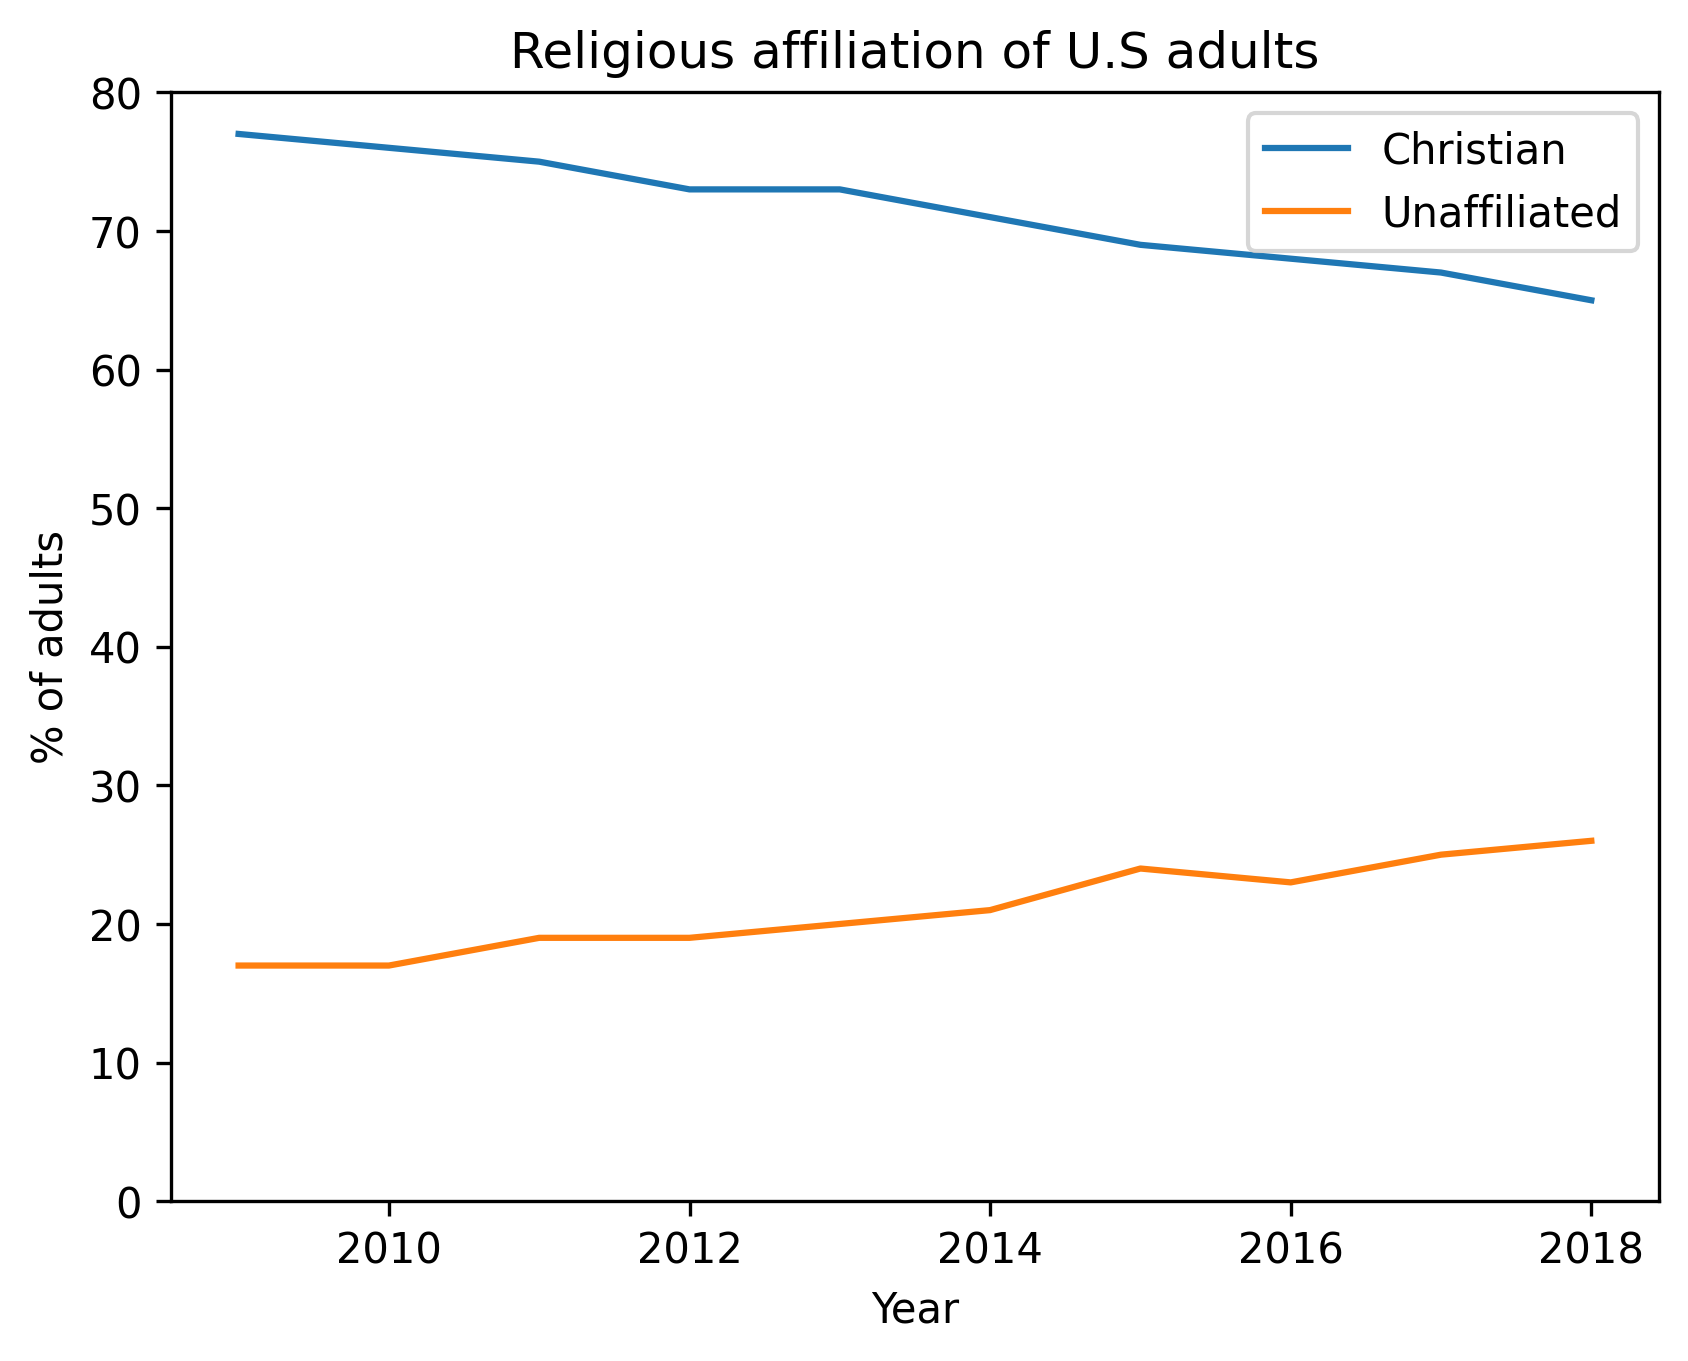
\includegraphics[width=4in]{chapters/06_plotting_files/06_plotting_31_0.png}
\end{center}

Now let's add another important element, a legend that indicates which
line is which. To do that, we add a label to each line, using the
keyword argument \passthrough{\lstinline!label!}. Then we call
\passthrough{\lstinline!plt.legend!} to create the legend.

\begin{lstlisting}[]
plt.plot(year, christian, label='Christian')
plt.plot(year, unaffiliated, label='Unaffiliated')

plt.ylim([0, 80])
plt.xlabel('Year')
plt.ylabel('% of adults')
plt.title('Religious affiliation of U.S adults')
plt.legend();
\end{lstlisting}

\begin{center}
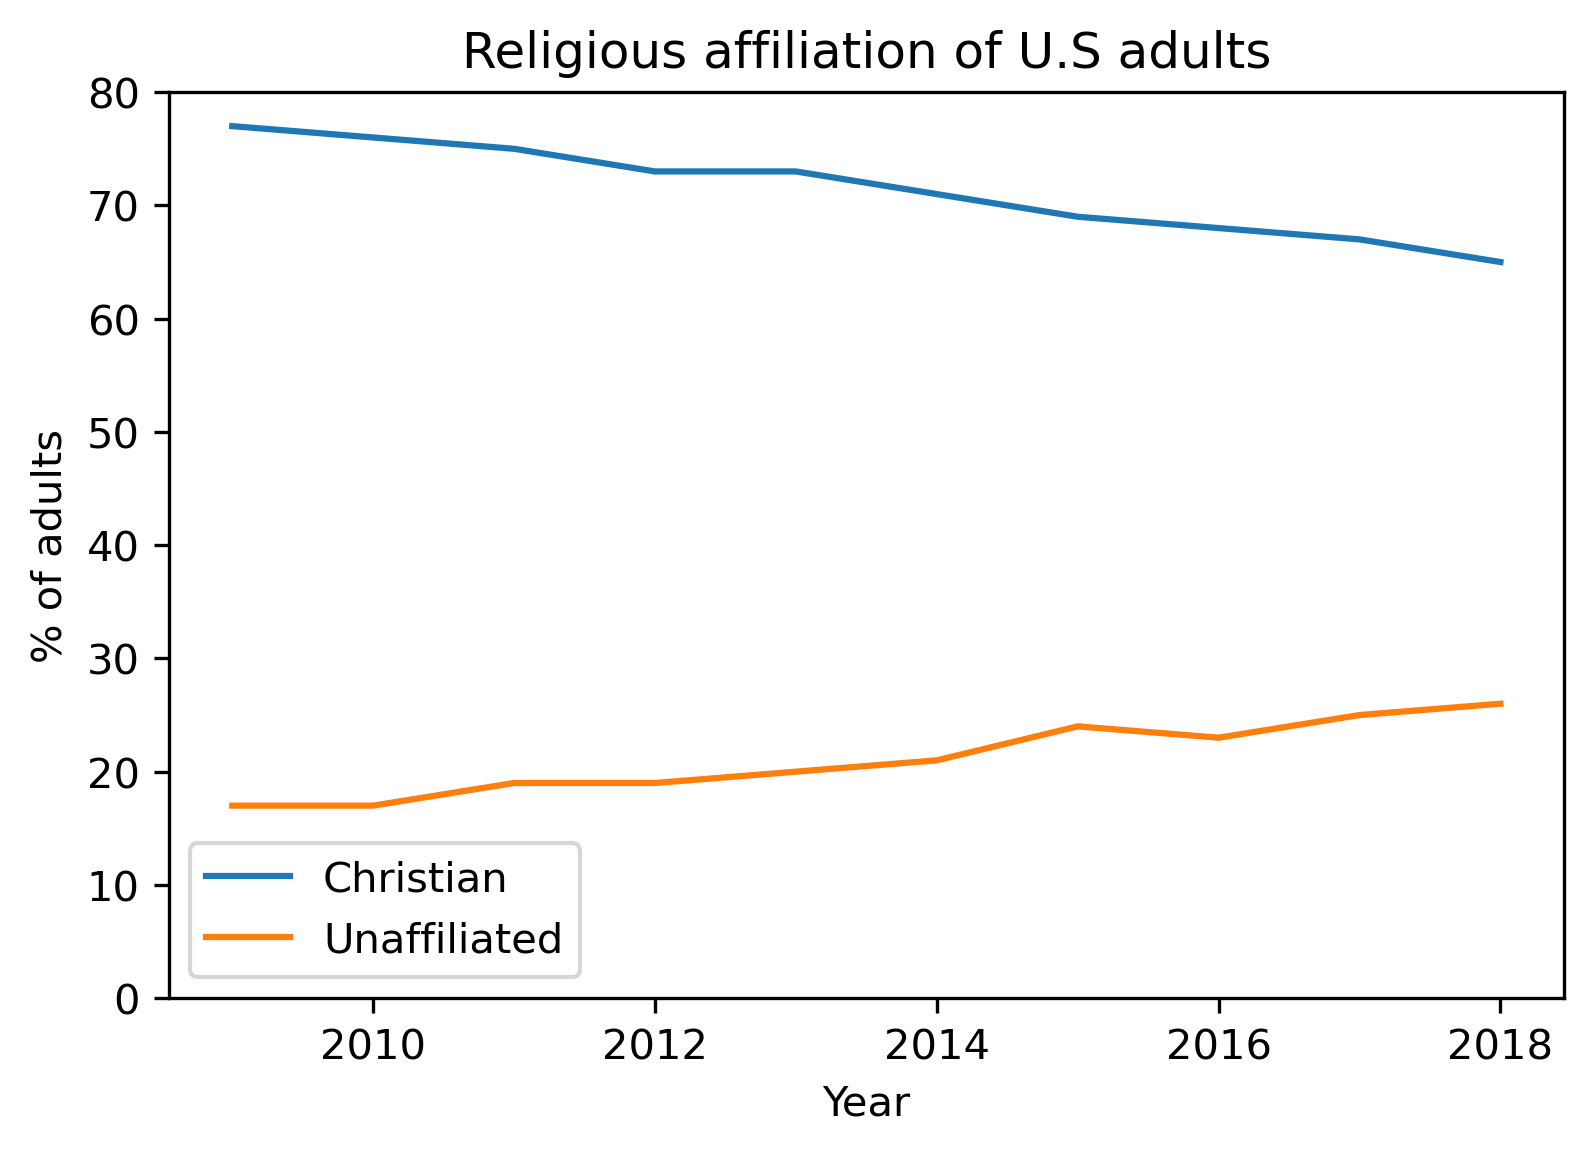
\includegraphics[width=4in]{chapters/06_plotting_files/06_plotting_33_0.png}
\end{center}

\textbf{Exercise:} The orginal figure plots lines between the data
points, but it also plots ``markers'' showing the location of each data
point. It is generally good practice to include markers, especially if
data are not available for every year.

Modify the previous example to include a keyword argument
\passthrough{\lstinline!marker!} with the string value
\passthrough{\lstinline!'o'!}, which indicates that you want to plot
circles as markers.

\textbf{Exercise:} In the original figure, the line labelled
\passthrough{\lstinline!'Christian'!} is red and the line labeled
\passthrough{\lstinline!'Unaffiliated'!} is grey.

Find the online documentation of \passthrough{\lstinline!plt.plot!} and
figure out how to use keyword arguments to specify colors. Choose colors
to (roughly) match the original figure.

The \passthrough{\lstinline!legend!} function takes a keyword argument
that speficies the location of the legend. Read the documentation of
this function and move the legend to the center left of the figure.

\hypertarget{sandwiches}{%
\section{Sandwiches}\label{sandwiches}}

In a previous chapter we used data from an article in \emph{The
Economist} comparing sandwich prices in Boston and London: ``Why
Americans pay more for lunch than Britons do'' at
\url{https://www.economist.com/finance-and-economics/2019/09/07/why-americans-pay-more-for-lunch-than-britons-do}.

The article includes this graph showing prices of several sandwiches in
the two cities:

As an exercise, let's see if we can replicate this figure. Here's the
data from the article again: the names of the sandwiches and the price
list for each city.

\begin{lstlisting}[]
name_list = [
    'Lobster roll',
    'Chicken caesar',
    'Bang bang chicken',
    'Ham and cheese',
    'Tuna and cucumber',
    'Egg'
]

boston_price_list = [9.99, 7.99, 7.49, 7, 6.29, 4.99]
london_price_list = [7.5, 5, 4.4, 5, 3.75, 2.25]
\end{lstlisting}

In the previous section we plotted percentages on the
\passthrough{\lstinline!y!} axis versus time on the
\passthrough{\lstinline!x!} axis. Now we want to plot the sandwich names
on the \passthrough{\lstinline!y!} axis and the prices on the
\passthrough{\lstinline!x!} axis. Here's how:

\begin{lstlisting}[]
plt.plot(boston_price_list, name_list)
plt.xlabel('Price in USD');
\end{lstlisting}

\begin{center}
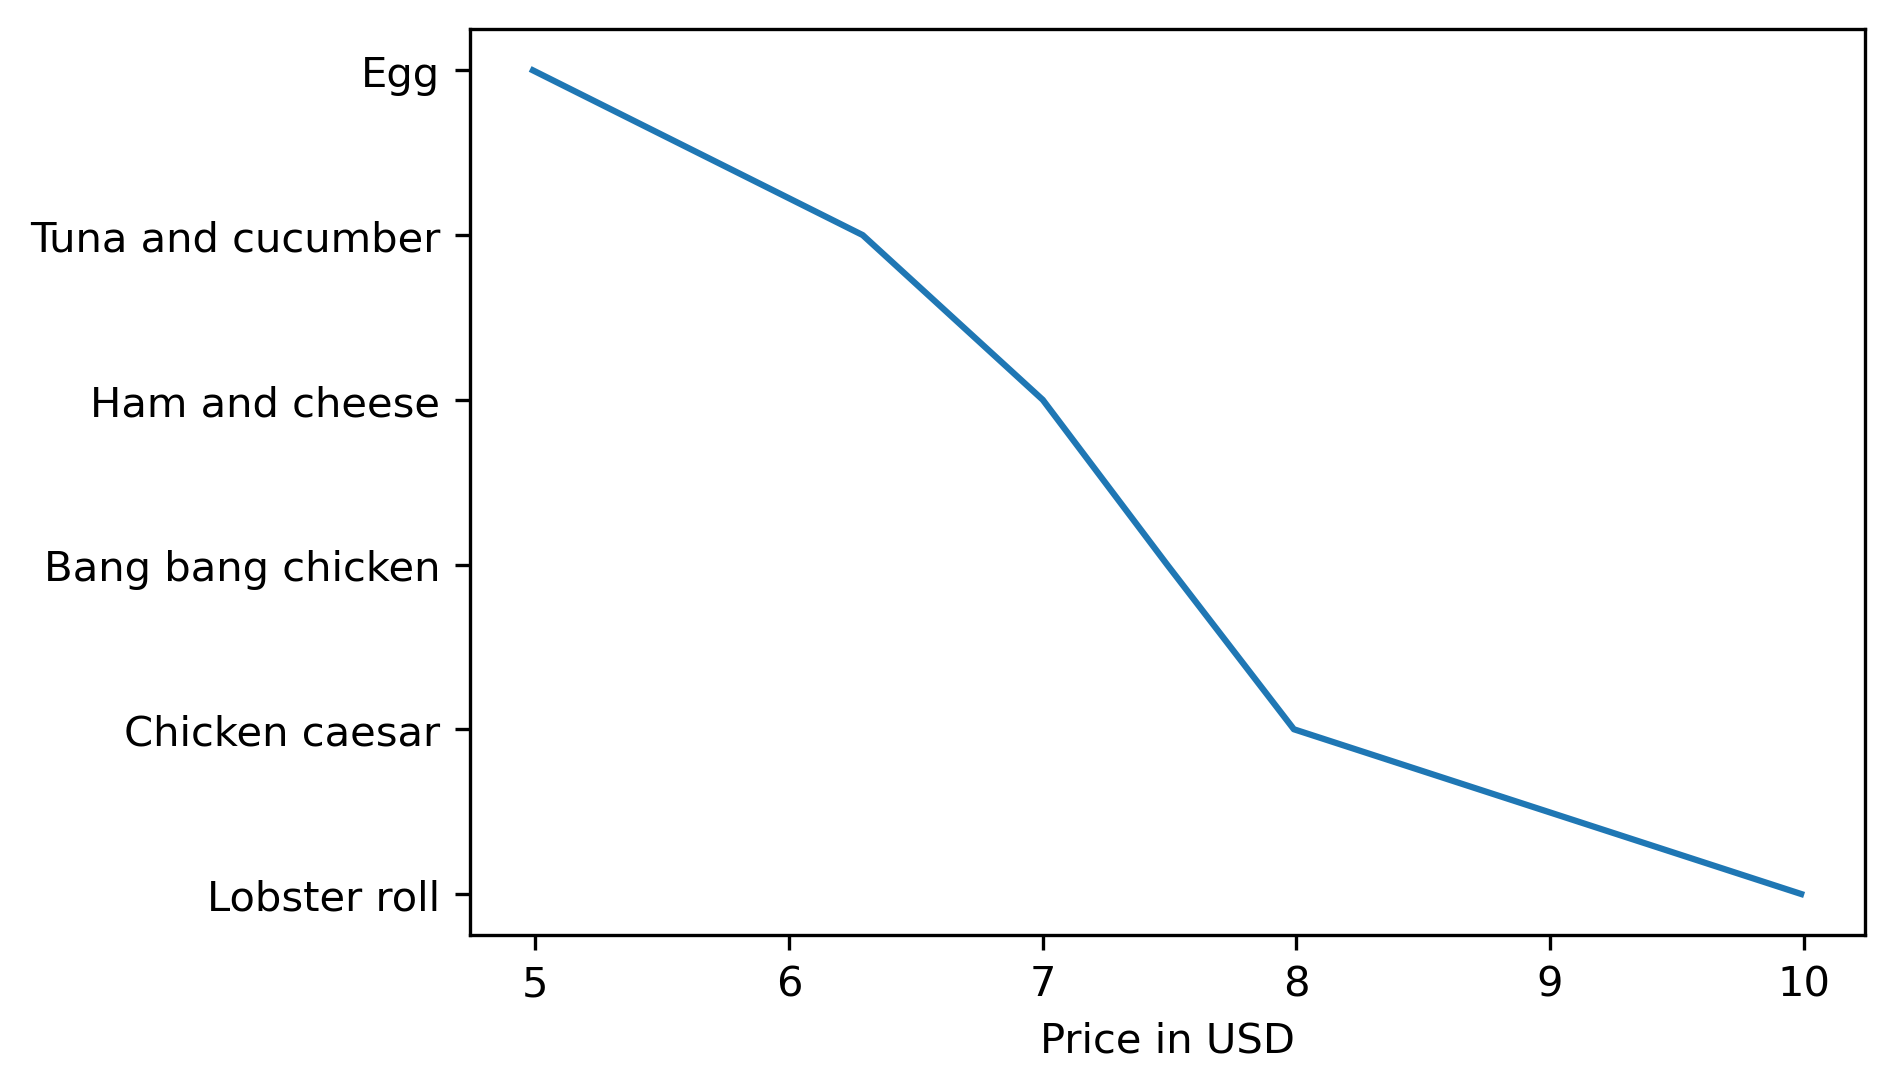
\includegraphics[width=4in]{chapters/06_plotting_files/06_plotting_39_0.png}
\end{center}

\passthrough{\lstinline!name\_list!} is a list of strings; Pyplot orders
them from top to bottom, equally spaced.

By default Pyplot connects the points with lines, but in this example
the lines don't make sense because the sandwich names are
\textbf{categorical}, not numerical. You can't interpolate between an
egg sandwich and a tuna sandwich.

We can turn on markers and turn off lines with keyword arguments.

\begin{lstlisting}[]
plt.plot(boston_price_list, name_list, 
         marker='o', linestyle='')
plt.xlabel('Price in USD');
\end{lstlisting}

\begin{center}
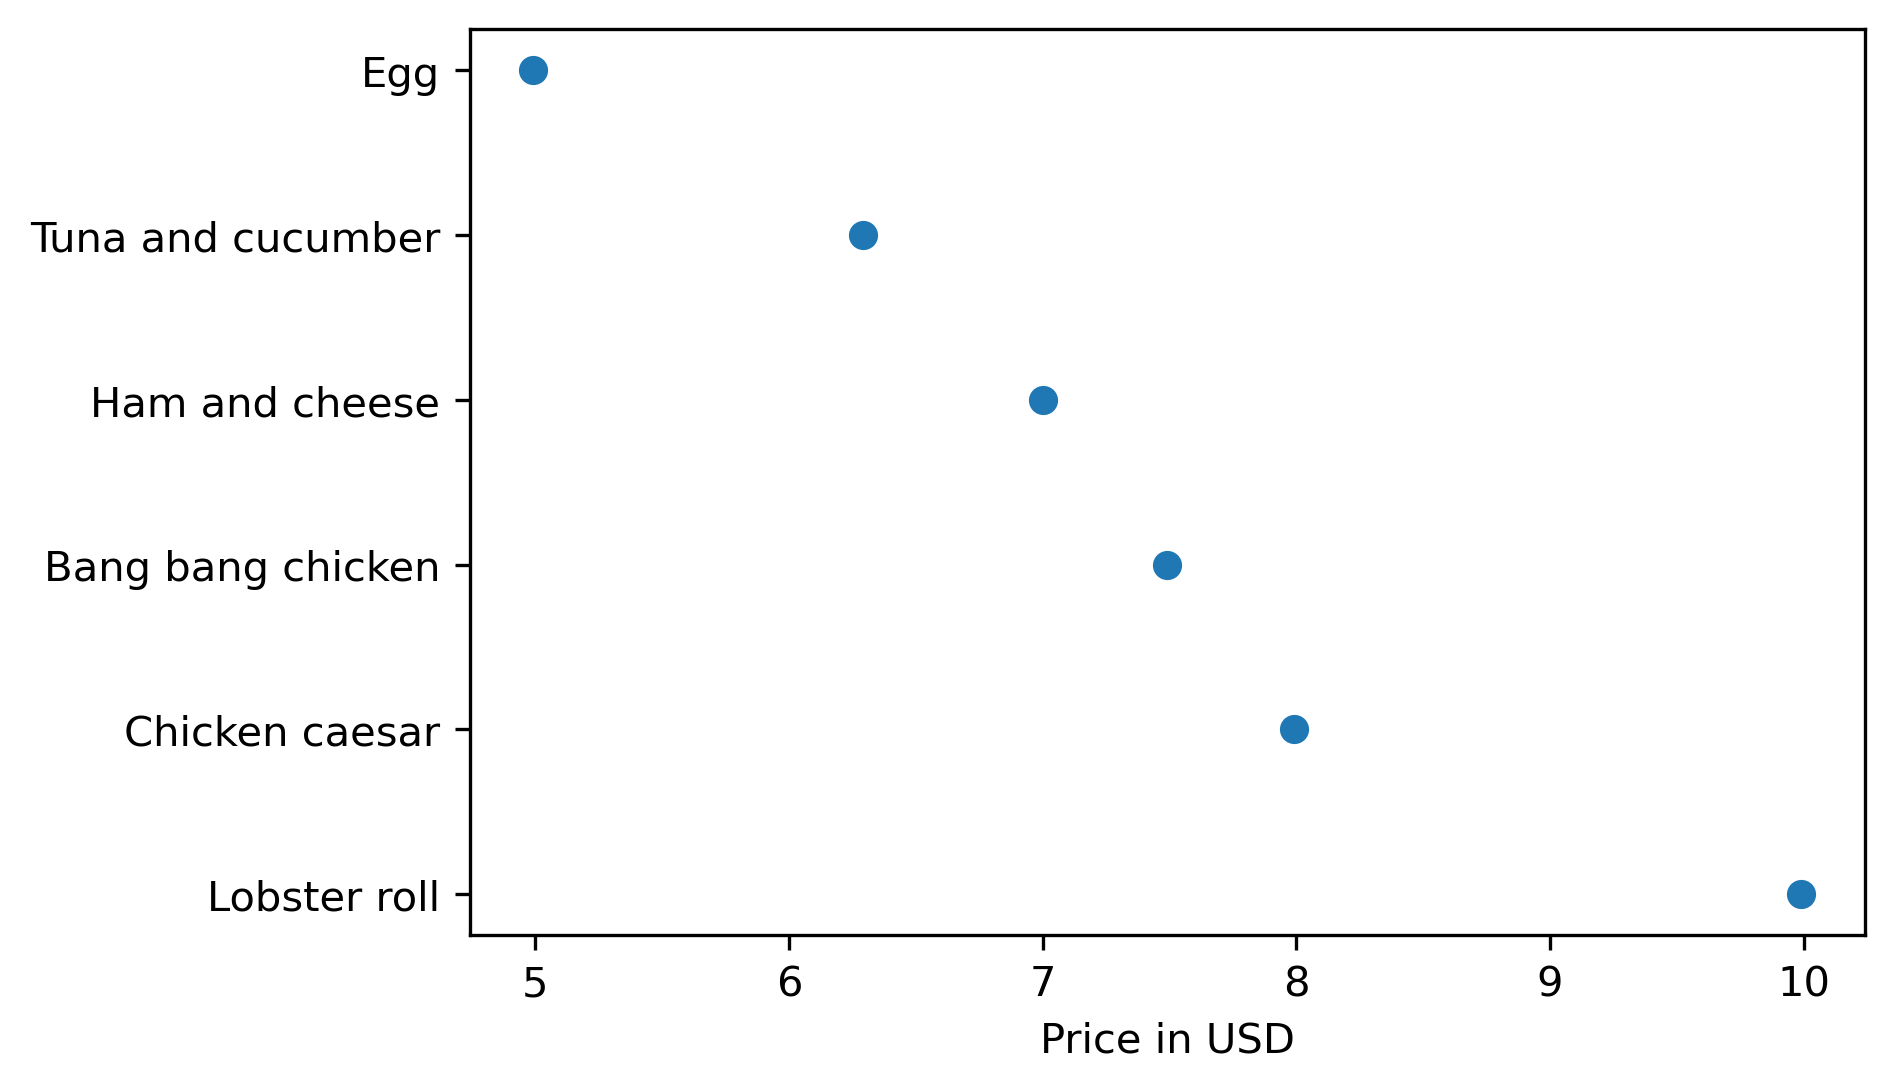
\includegraphics[width=4in]{chapters/06_plotting_files/06_plotting_41_0.png}
\end{center}

Or we can do the same thing more concisely by providing a \textbf{format
string} as a positional argument. You can read the documentation of
\passthrough{\lstinline!plt.plot!} to learn more about format strings.

\begin{lstlisting}[]
plt.plot(boston_price_list, name_list, 'o')
plt.plot(london_price_list, name_list, 's')

plt.xlabel('Price in USD')
plt.title('Pret a Manger prices in Boston and London');
\end{lstlisting}

\begin{center}
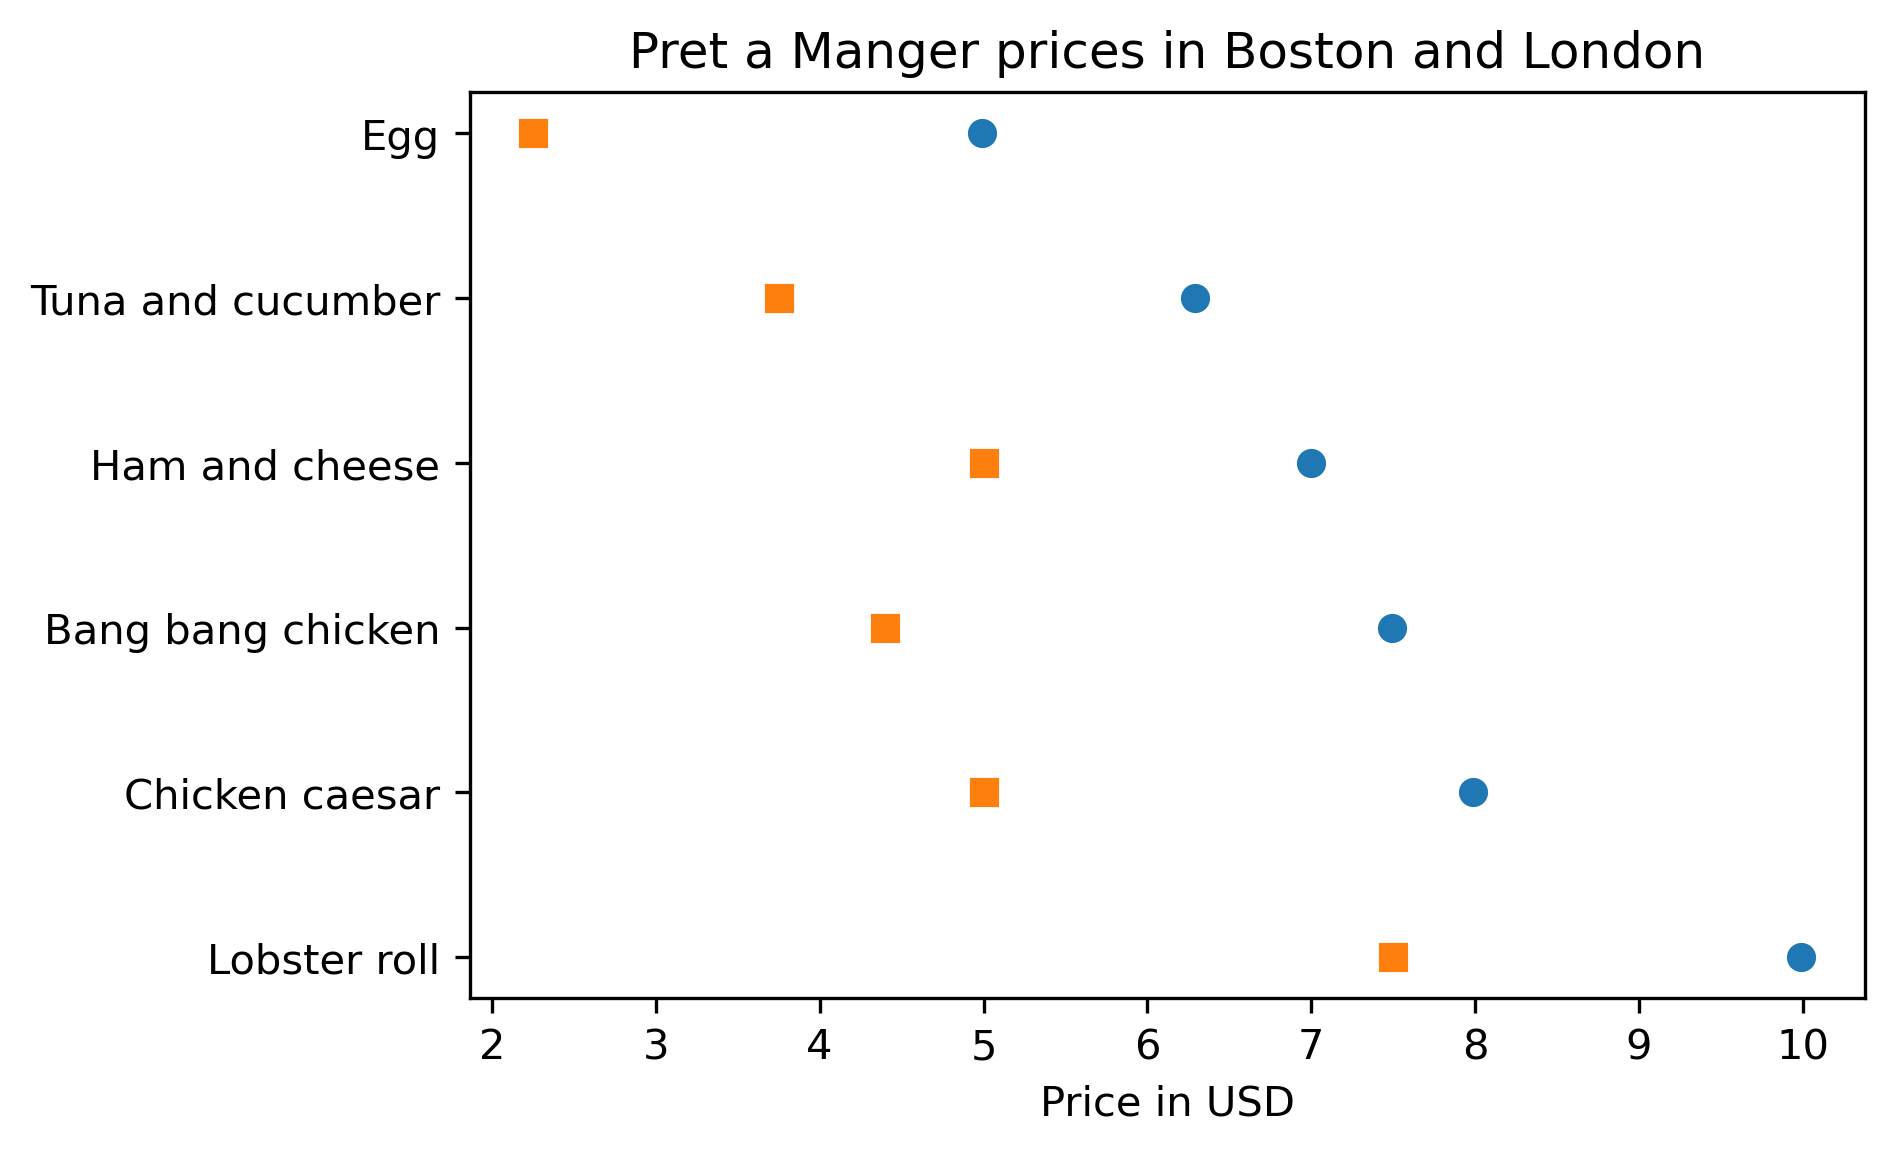
\includegraphics[width=4in]{chapters/06_plotting_files/06_plotting_43_0.png}
\end{center}

I added a title at the same time.

Now, to approximate the colors in the original figure, we can use the
strings \passthrough{\lstinline!'C3'!} and
\passthrough{\lstinline!'C0'!}, which specify colors from the default
color sequence. You can read the documentation to learn more about
specifying colors in Pyplot:
\url{https://matplotlib.org/3.1.1/tutorials/colors/colors.html}.

\begin{lstlisting}[]
plt.plot(boston_price_list, name_list, 'o', color='C3')
plt.plot(london_price_list, name_list, 's', color='C0')

plt.xlabel('Price in USD')
plt.title('Pret a Manger prices in Boston and London');
\end{lstlisting}

\begin{center}
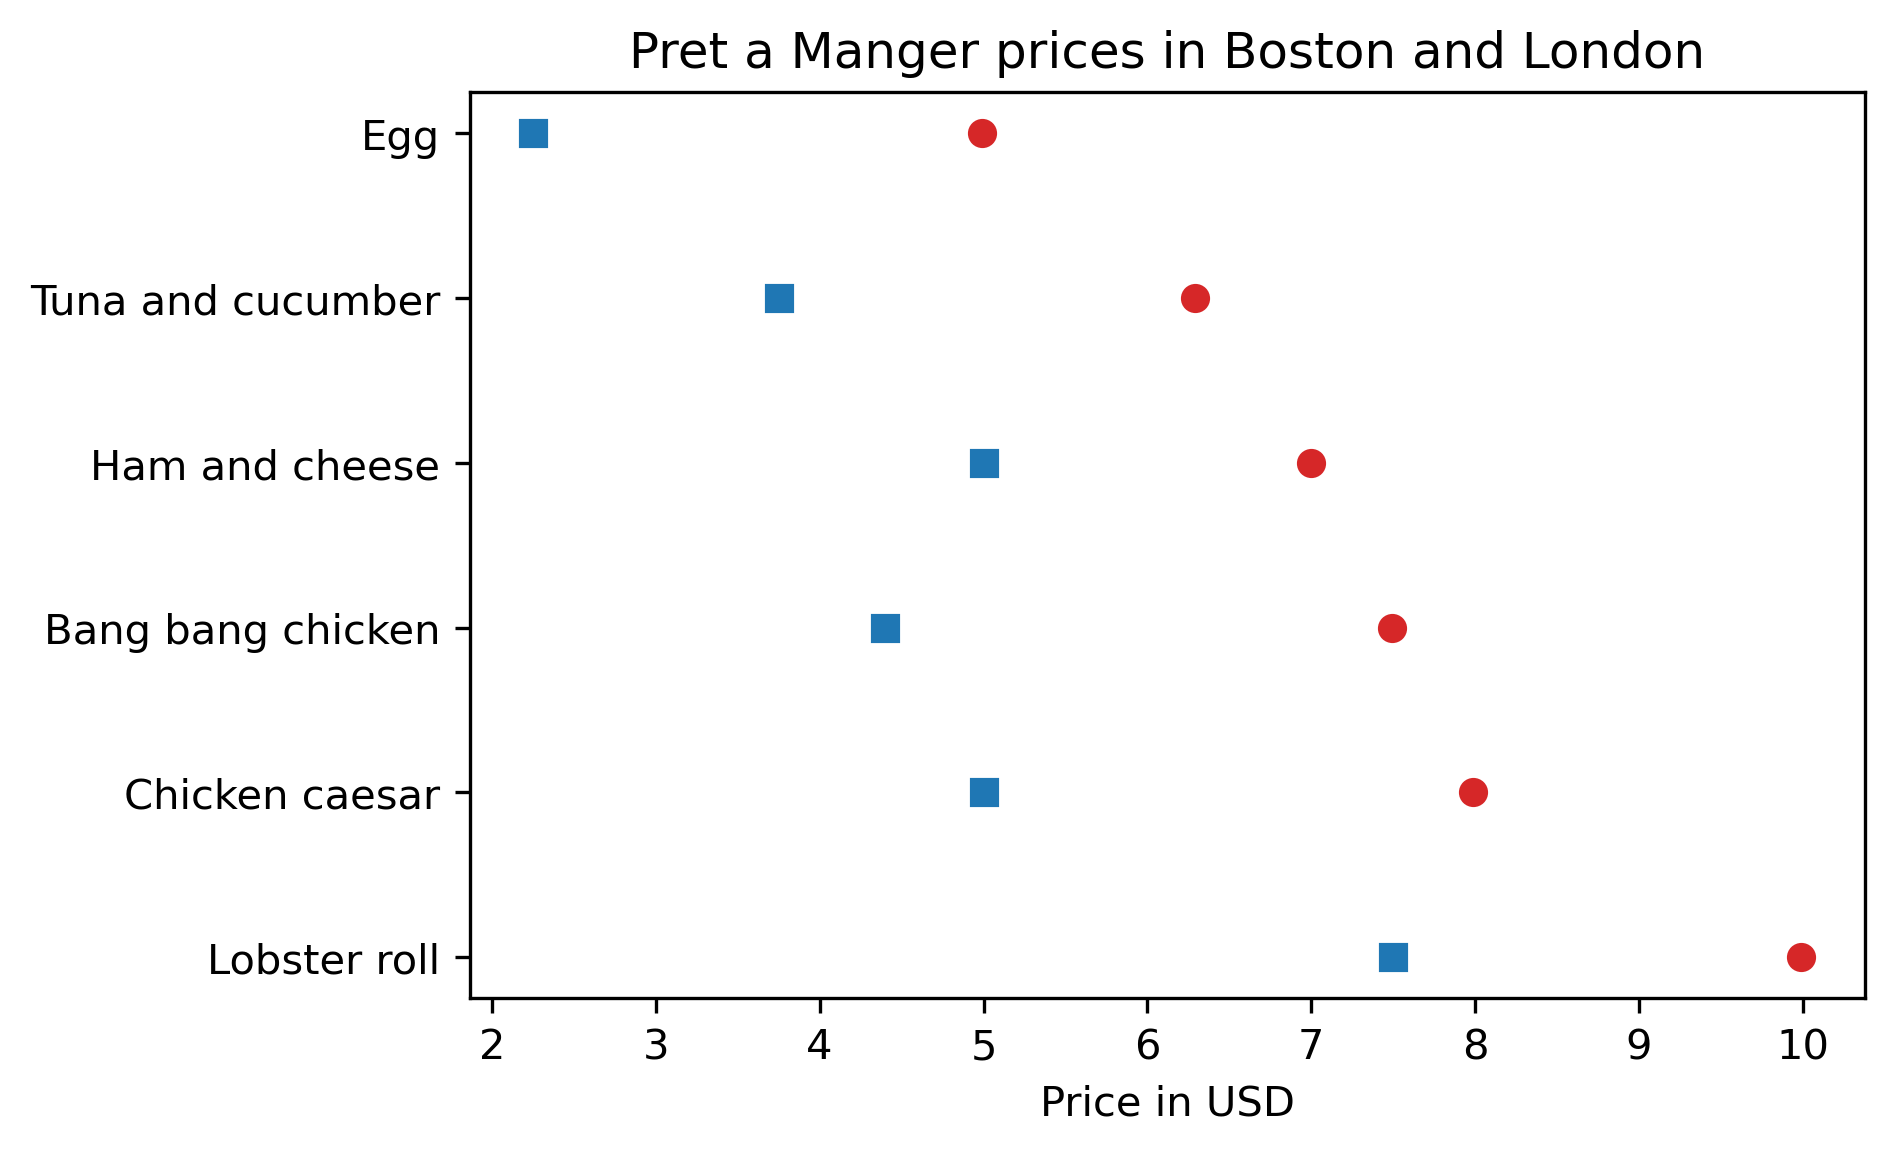
\includegraphics[width=4in]{chapters/06_plotting_files/06_plotting_45_0.png}
\end{center}

To connect the dots with lines, we'll use
\passthrough{\lstinline!plt.hlines!}, which draws horizontal lines. It
takes three arguments: a sequence of values on the
\passthrough{\lstinline!y!} axis, which are the sandwich names in this
example, and two sequences of values on the \passthrough{\lstinline!x!}
axis, which are the London prices and Boston prices.

\begin{lstlisting}[]
plt.plot(boston_price_list, name_list, 'o', color='C3')
plt.plot(london_price_list, name_list, 's', color='C0')

plt.hlines(name_list, london_price_list, boston_price_list)

plt.xlabel('Price in USD')
plt.title('Pret a Manger prices in Boston and London');
\end{lstlisting}

\begin{center}
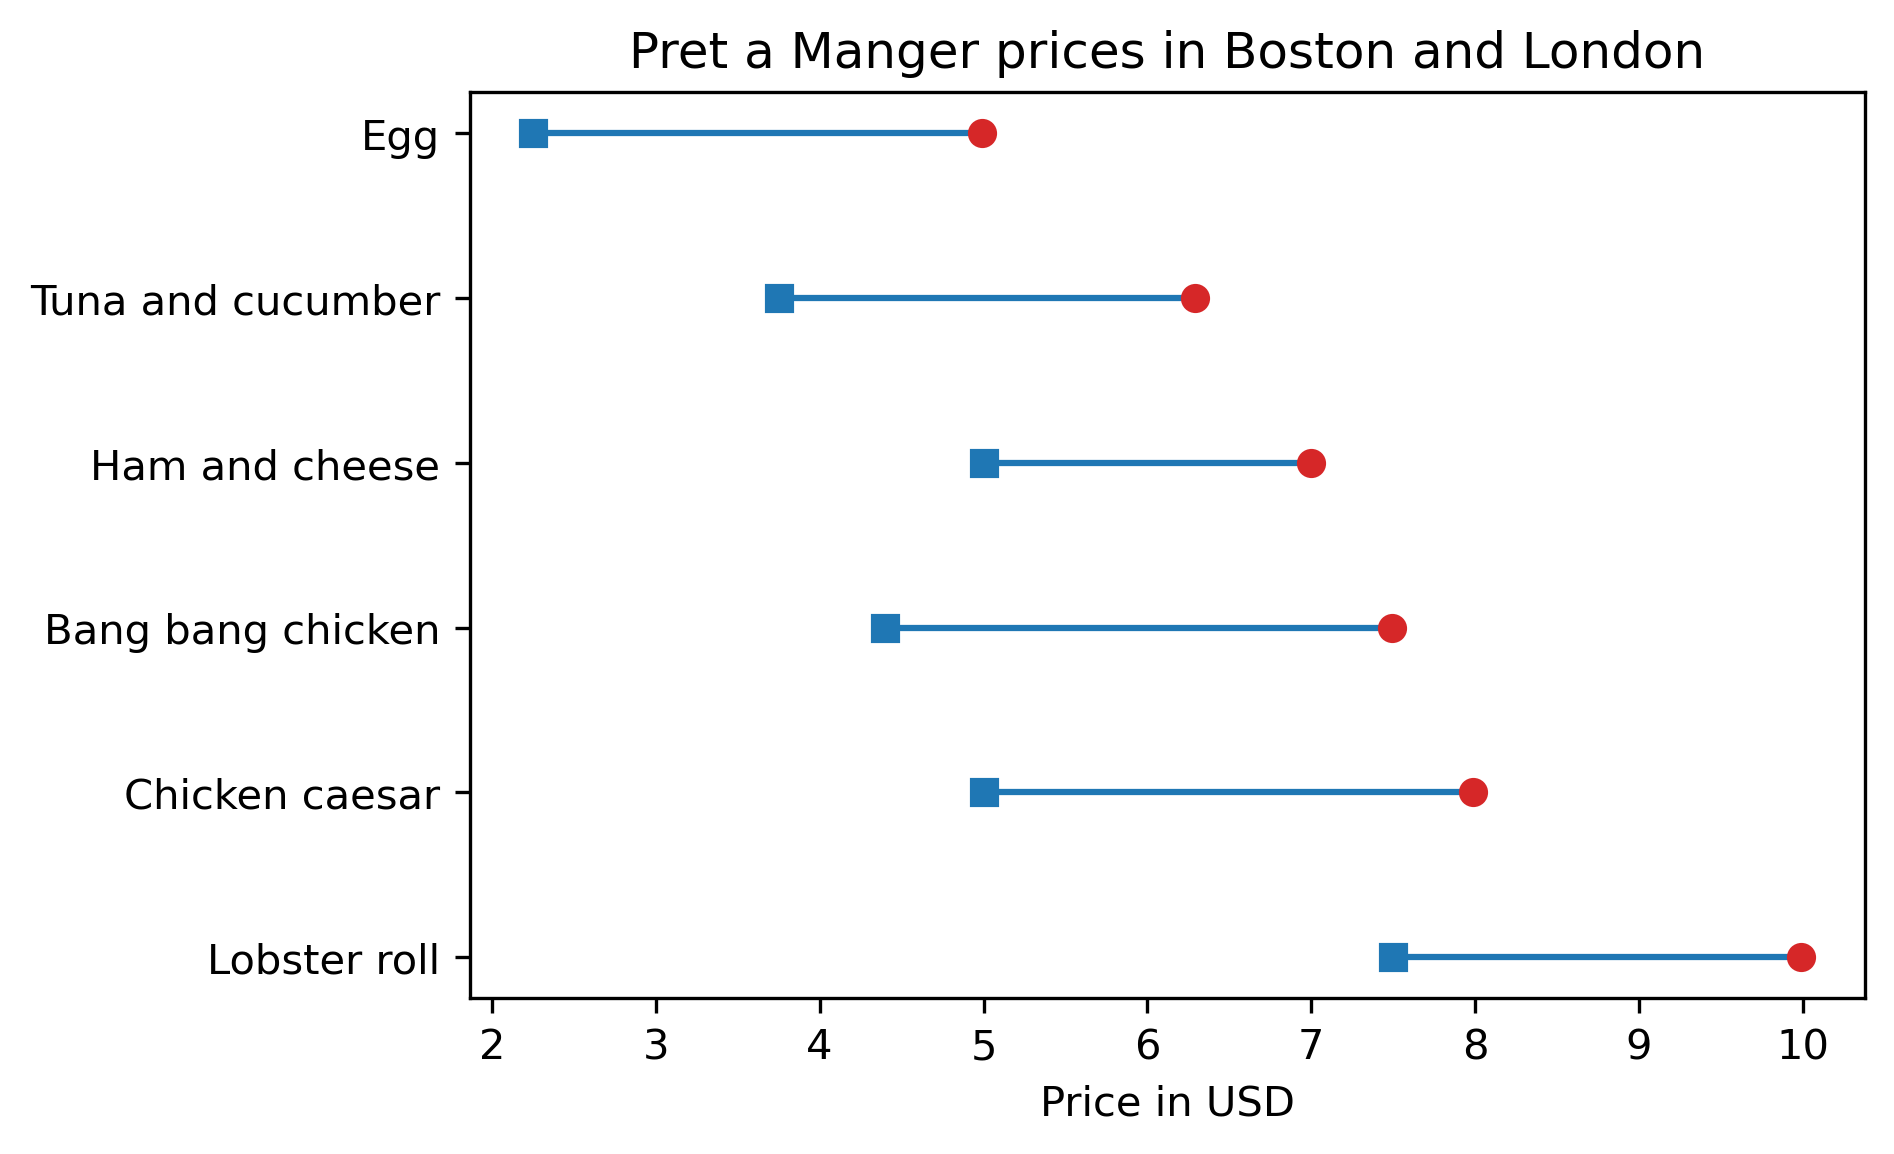
\includegraphics[width=4in]{chapters/06_plotting_files/06_plotting_47_0.png}
\end{center}

\textbf{Exercise:} To finish off this example, add a legend that
identifies the London and Boston prices. Remember that you have to add a
\passthrough{\lstinline!label!} keyword each time you call
\passthrough{\lstinline!plt.plot!}, and then call
\passthrough{\lstinline!plt.legend!}.

Notice that the sandwiches in our figure are in the opposite order of
the sandwiches in the original figure. There is a Pyplot function that
inverts the \passthrough{\lstinline!y!} axis; see if you can find it and
use it to reverse the order of the sandwich list.

\hypertarget{zipfs-law}{%
\section{Zipf's Law}\label{zipfs-law}}

In the previous chapter we downloaded \emph{War and Peace} from Project
Gutenberg and counted the number of lines and words. Then we used a
dictionary to count the number of unique words and the number of times
each one appears. Now we'll use those results to generate a ``Zipf
plot'', which shows the frequency of the words on the
\passthrough{\lstinline!y!} axis, ordered from the most common word to
the least.

In the previous chapter, we looped through the book and made a string
that contains all punctuation characters. Here are the results, which we
will need again.

\begin{lstlisting}[]
all_punctuation = ',.-:[#]*/“’—‘!?”;()%@'
\end{lstlisting}

And here's a solution to one of the previous exercises. It loops through
the book and makes a dictionary that maps from each word to the number
of times it appears.

\begin{lstlisting}[]
first_line = "CHAPTER I\n"
last_line = ("End of the Project Gutenberg EBook of " +
             "War and Peace, by Leo Tolstoy\n")

fp = open('2600-0.txt')
for line in fp:
    if line == first_line:
        break

unique_words = {}
for line in fp:
    if line == last_line:
        break
        
    for word in line.split():
        word = word.lower()
        word = word.strip(all_punctuation)
        if word in unique_words:
            unique_words[word] += 1
        else:
            unique_words[word] = 1
\end{lstlisting}

\hypertarget{frequencies-and-ranks}{%
\section{Frequencies and Ranks}\label{frequencies-and-ranks}}

In this section we'll test Zipf's law, which states that

\begin{quote}
given some corpus of natural language utterances, the frequency of any
word is inversely proportional to its rank in the frequency table. Thus
the most frequent word will occur approximately twice as often as the
second most frequent word, three times as often as the third most
frequent word, etc.
\end{quote}

See \url{https://en.wikipedia.org/wiki/Zipfs_law}. To see if this law
holds for the words in \emph{War and Peace}, we'll make a plot that
shows:

\begin{itemize}
\item
  The frequency of each word on the \passthrough{\lstinline!y!} axis,
  and
\item
  The rank of each word on the \passthrough{\lstinline!x!} axis, where
  the rank of the most frequent word is 1, the rank of the second most
  common word is 2, etc.
\end{itemize}

In \passthrough{\lstinline!unique\_words!}, the keys are words and the
values are their frequencies. We can use the
\passthrough{\lstinline!values!} function to get the values from the
dictionary. The result has the type
\passthrough{\lstinline!dict\_values!}:

\begin{lstlisting}[]
freqs = unique_words.values()
type(freqs)
(@\dashfill@)
@@@dict_values@@@
\end{lstlisting}

Before we plot them, we have to sort them, but the
\passthrough{\lstinline!sort!} function doesn't work with
\passthrough{\lstinline!dict\_values!}.

We can use \passthrough{\lstinline!list!} to make a list of frequencies:

\begin{lstlisting}[]
freqs = list(unique_words.values())
type(freqs)
(@\dashfill@)
@@@list@@@
\end{lstlisting}

And now we can use \passthrough{\lstinline!sort!}. By default it sorts
in ascending order, but we can pass a keyword argument to reverse the
order.

\begin{lstlisting}[]
freqs.sort(reverse=True)
\end{lstlisting}

Now, for the ranks, we need a sequence that counts from 1 to
\passthrough{\lstinline!n!}, where \passthrough{\lstinline!n!} is the
number of elements in \passthrough{\lstinline!freqs!}. We can use the
\passthrough{\lstinline!range!} function, which returns a value with
type \passthrough{\lstinline!range!}.

As a small example, here's the range from 1 to 5.

\begin{lstlisting}[]
range(1, 5)
(@\dashfill@)
@@@range(1, 5)@@@
\end{lstlisting}

However, there's a catch. If we use the range to make a list, we see
that ``the range from 1 to 5'' includes 1, but it doesn't include 5.

\begin{lstlisting}[]
list(range(1, 5))
(@\dashfill@)
@@@[1, 2, 3, 4]@@@
\end{lstlisting}

That might seem strange, but it is often more convenient to use
\passthrough{\lstinline!range!} when it is defined this way, rather than
what might seem like the more natural way (see
\url{https://www.cs.utexas.edu/users/EWD/transcriptions/EWD08xx/EWD831.html}).
Anyway, we can get what we want by increasing the second argument by
one:

\begin{lstlisting}[]
list(range(1, 6))
(@\dashfill@)
@@@[1, 2, 3, 4, 5]@@@
\end{lstlisting}

So, finally, we can make a range that represents the ranks from
\passthrough{\lstinline!1!} to \passthrough{\lstinline!n!}:

\begin{lstlisting}[]
n = len(freqs)
ranks = range(1, n+1)
ranks
(@\dashfill@)
@@@range(1, 20479)@@@
\end{lstlisting}

And now we can plot the frequencies versus the ranks:

\begin{lstlisting}[]
plt.plot(ranks, freqs)

plt.xlabel('Rank')
plt.ylabel('Frequency')
plt.title("War and Peace and Zipf's law");
\end{lstlisting}

\begin{center}
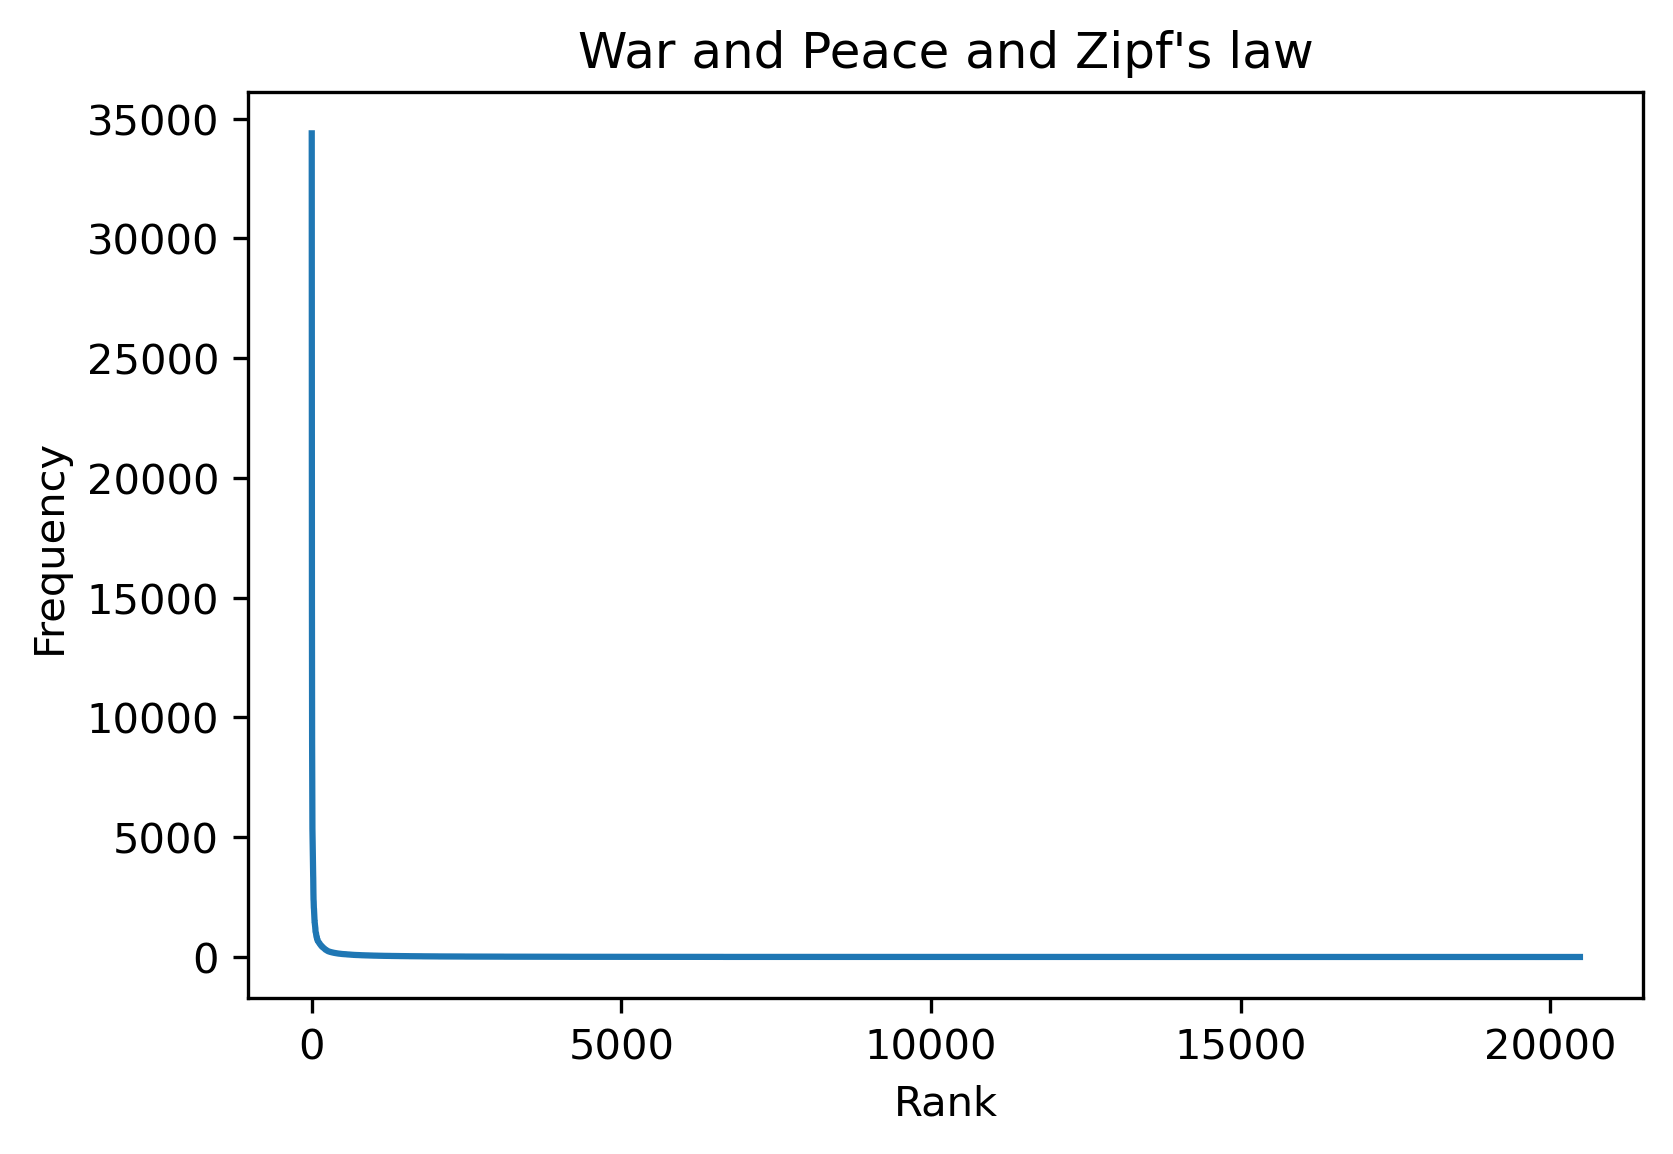
\includegraphics[width=4in]{chapters/06_plotting_files/06_plotting_74_0.png}
\end{center}

\hypertarget{logarithmic-scales}{%
\section{Logarithmic scales}\label{logarithmic-scales}}

The few most common words are very common, but the great majority of
words are rare. So that's consistent with Zipf's law, but Zipf's law is
more specific. It claims that the frequencies should be inversely
proportional to the ranks. If that's true, we can write:

\(f = k / r\)

where \(r\) is the rank of a word, \(f\) is its frequency, and \(k\) is
an unknown constant of proportionality. If we take the log of both
sides, we get this:

\(\log f = \log k - \log r\)

This equation implies that if we plot \(f\) versus \(r\) on a log-log
scale, we expect to see a straight line with intercept at \(\log k\) and
slope -1.

We can use \passthrough{\lstinline!plt.xscale!} to plot the
\passthrough{\lstinline!x!} axis on a log scale.

\begin{lstlisting}[]
plt.plot(ranks, freqs)

plt.xlabel('Rank')
plt.ylabel('Frequency')
plt.title("War and Peace and Zipf's law")
plt.xscale('log')
\end{lstlisting}

\begin{center}
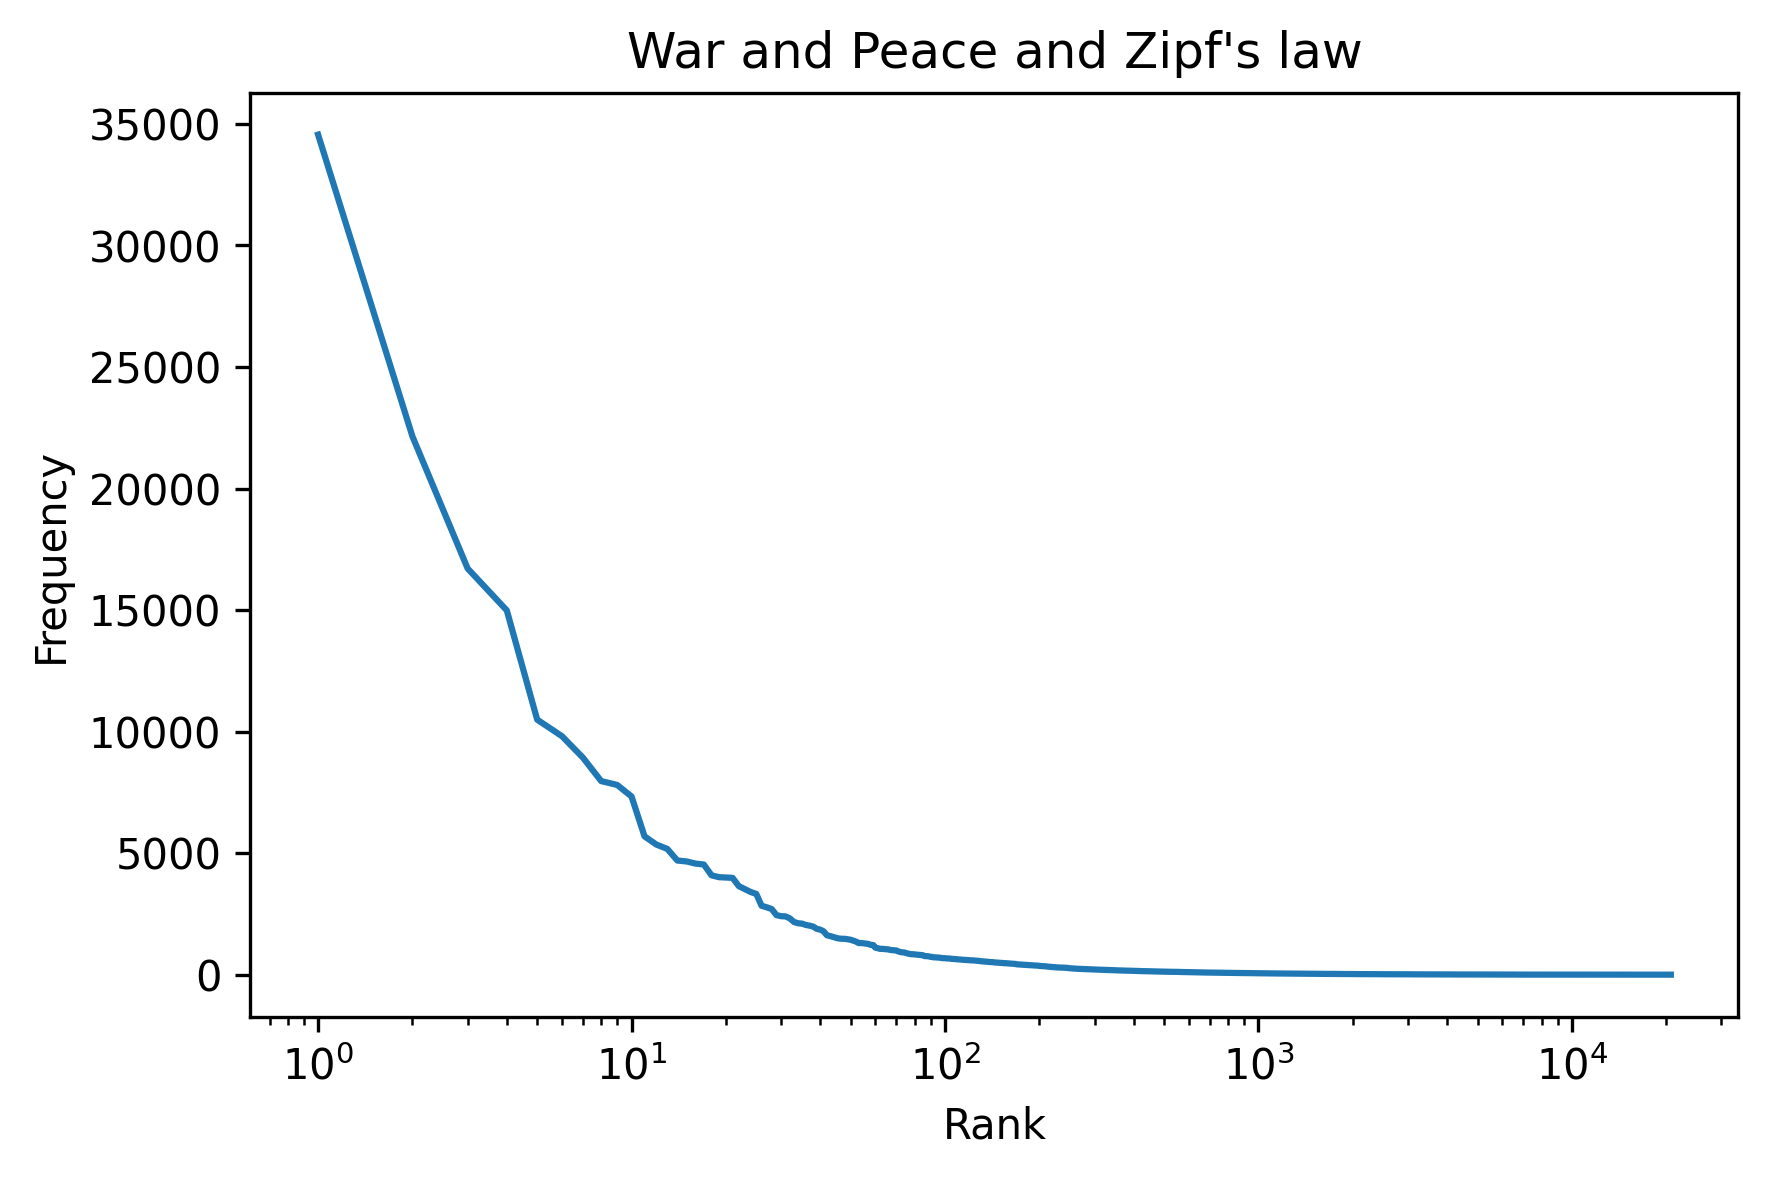
\includegraphics[width=4in]{chapters/06_plotting_files/06_plotting_76_0.png}
\end{center}

And \passthrough{\lstinline!plt.yscale!} to plot the
\passthrough{\lstinline!y!} axis on a log scale.

\begin{lstlisting}[]
plt.plot(ranks, freqs)

plt.xlabel('Rank')
plt.ylabel('Frequency')
plt.title("War and Peace and Zipf's law")
plt.xscale('log')
plt.yscale('log')
\end{lstlisting}

\begin{center}
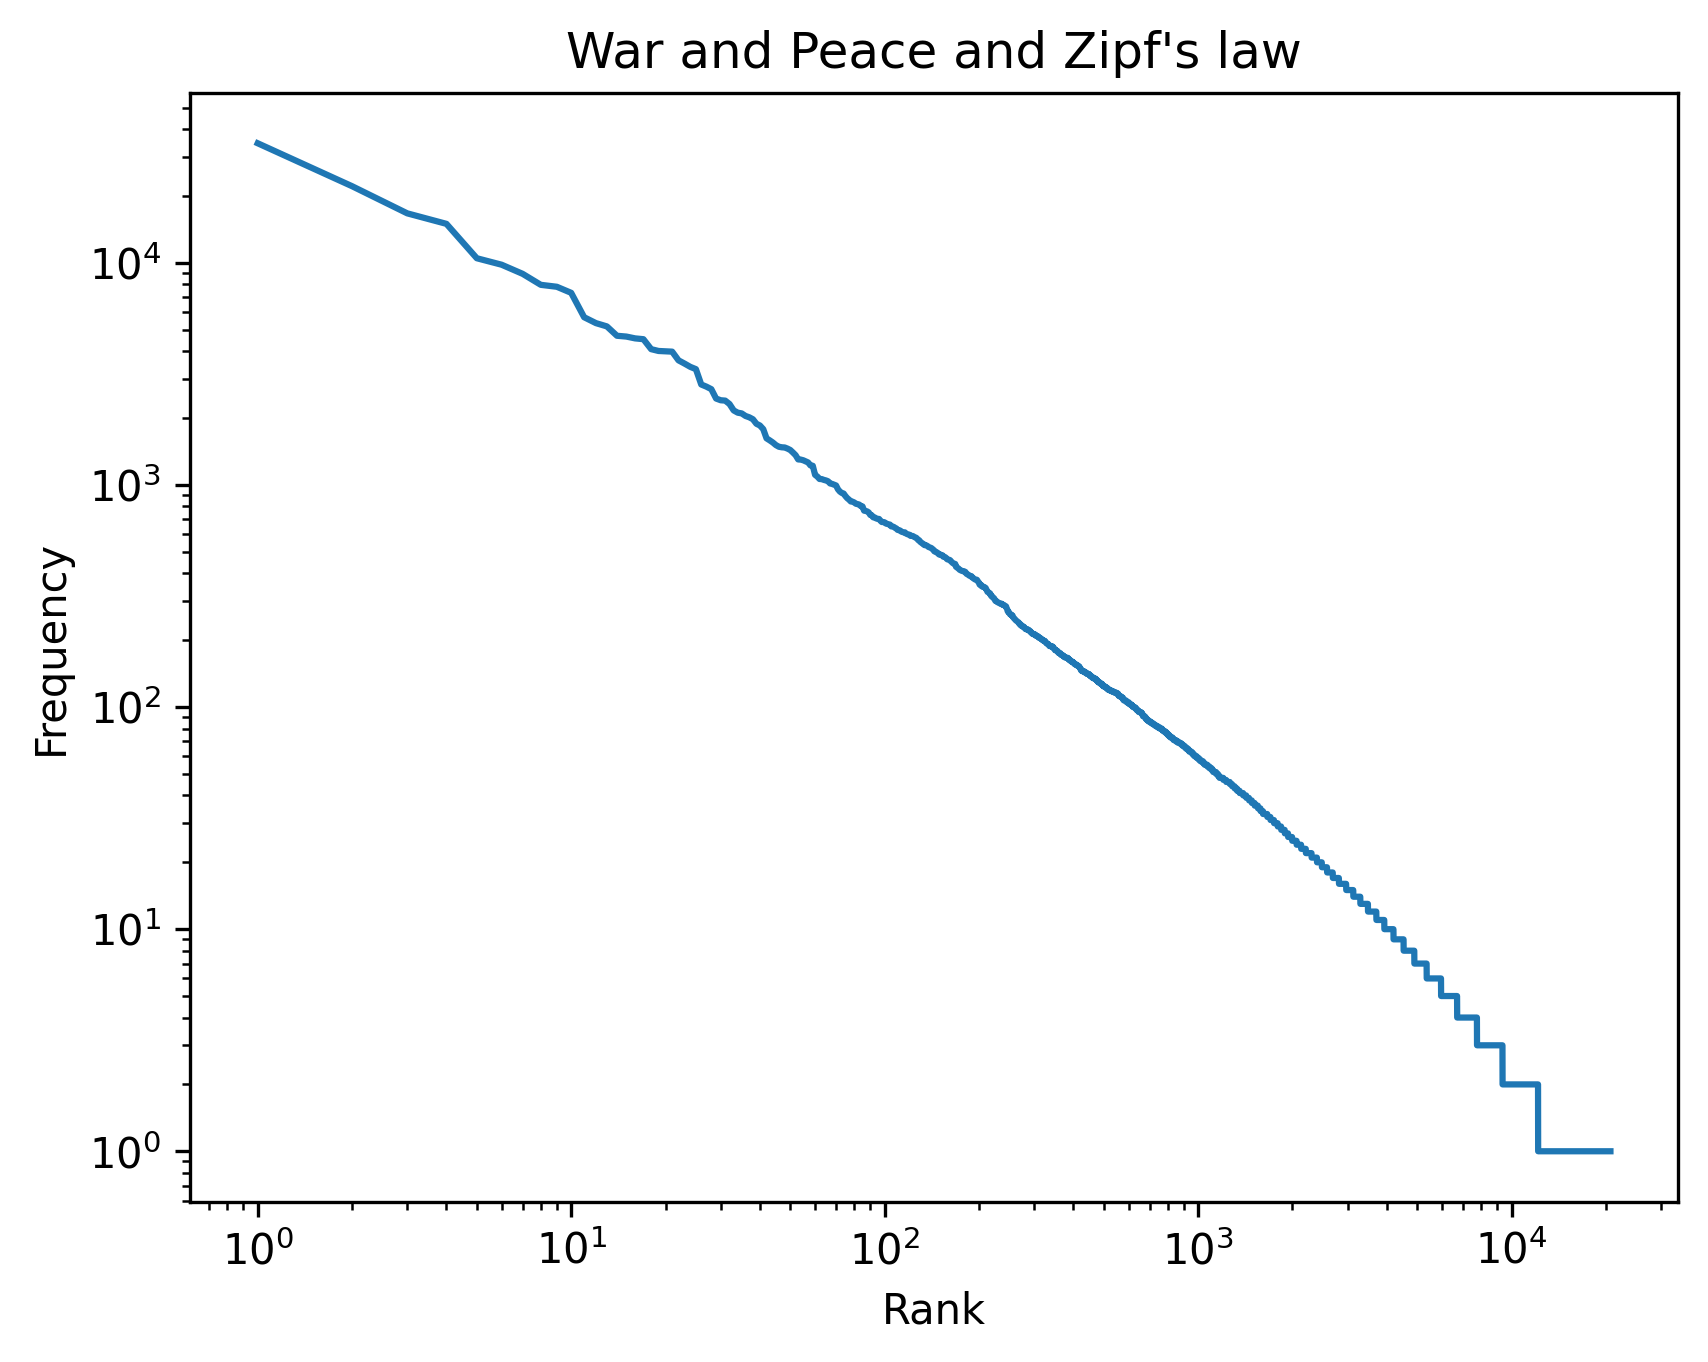
\includegraphics[width=4in]{chapters/06_plotting_files/06_plotting_78_0.png}
\end{center}

The result is not quite a straight line, but it is close. We can get a
sense of the slope by connecting the end points with a line. I'll select
the first and last elements from \passthrough{\lstinline!xs!}.

\begin{lstlisting}[]
xs = ranks[0], ranks[-1]
xs
(@\dashfill@)
@@@(1, 20478)@@@
\end{lstlisting}

And the first and last elements from \passthrough{\lstinline!ys!}.

\begin{lstlisting}[]
ys = freqs[0], freqs[-1]
ys
(@\dashfill@)
@@@(34388, 1)@@@
\end{lstlisting}

And plot a line between them.

\begin{lstlisting}[]
plt.plot(xs, ys, color='gray')
plt.plot(ranks, freqs)

plt.xlabel('Rank')
plt.ylabel('Frequency')
plt.title("War and Peace and Zipf's law")
plt.xscale('log')
plt.yscale('log')
\end{lstlisting}

\begin{center}
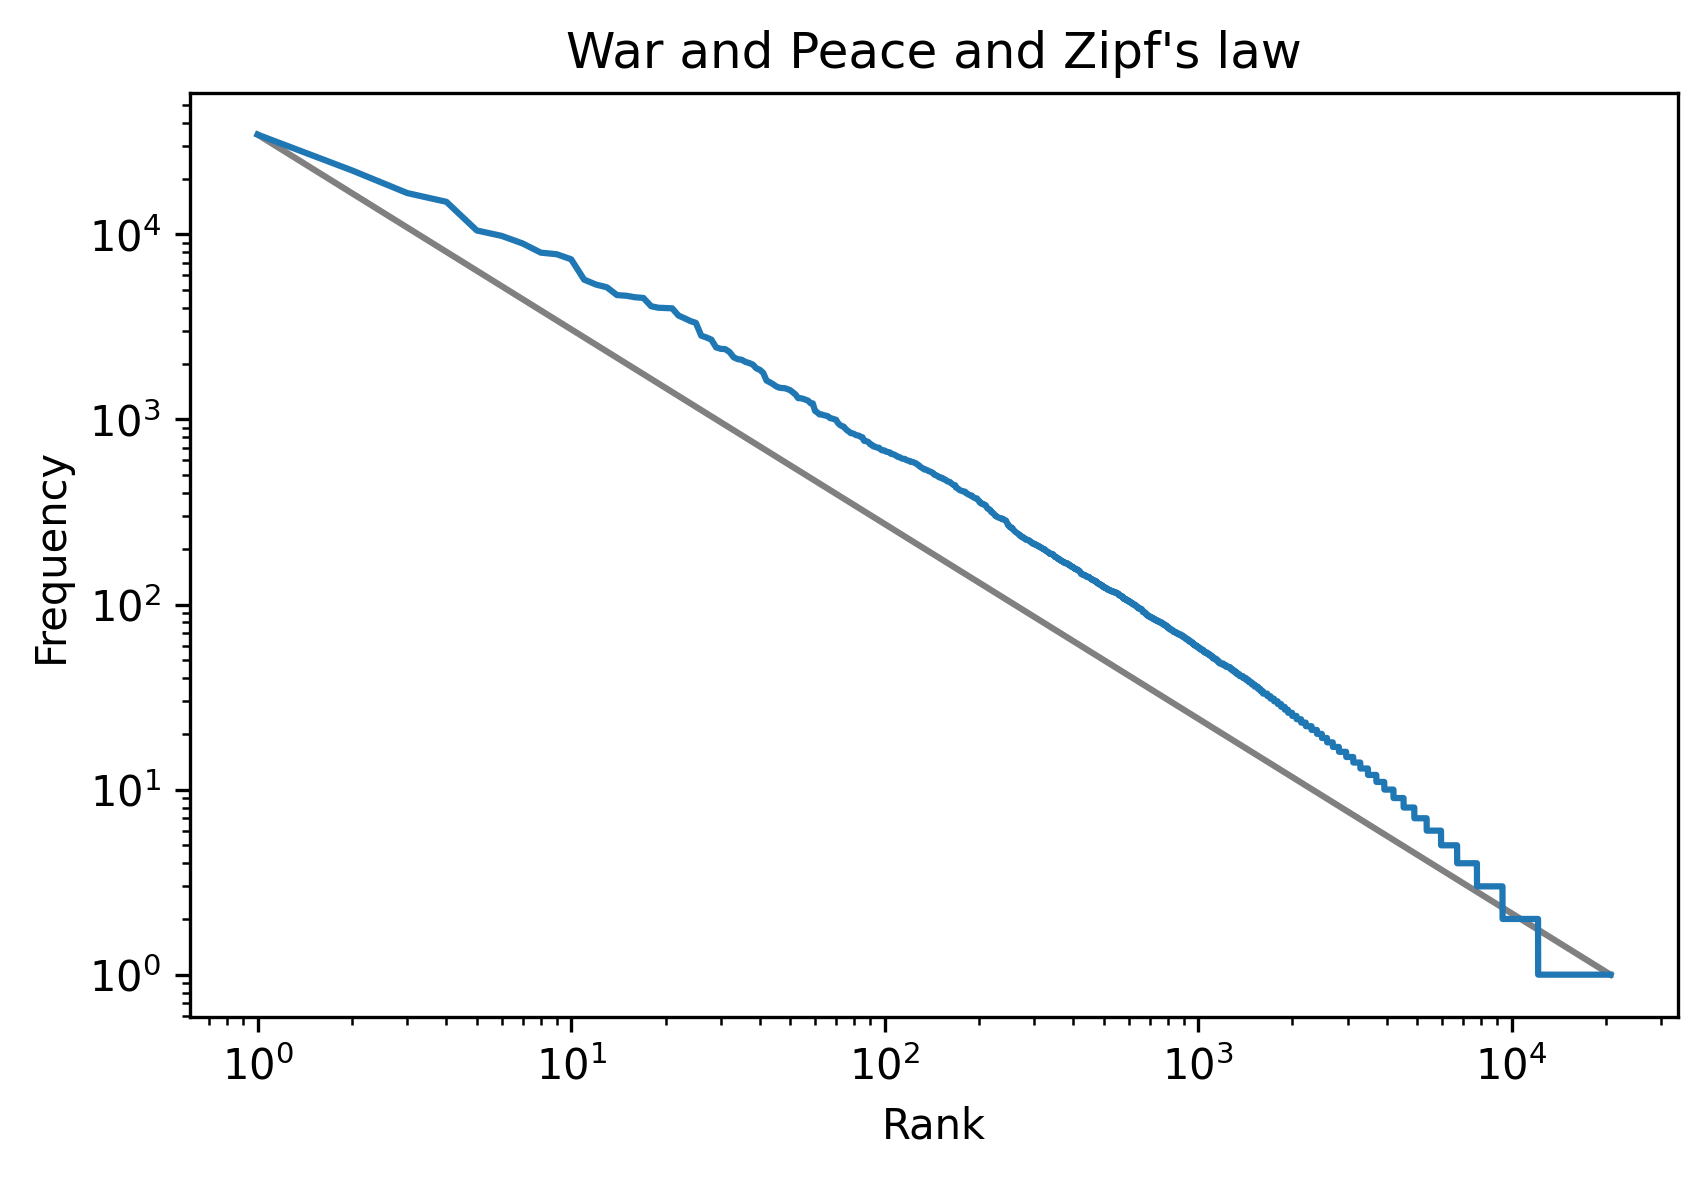
\includegraphics[width=4in]{chapters/06_plotting_files/06_plotting_84_0.png}
\end{center}

The slope of this line is the ``rise over run'', that is, the difference
on the \passthrough{\lstinline!y!} axis divided by the difference on the
\passthrough{\lstinline!x!} axis.

We can compute the rise using \passthrough{\lstinline!np.log10!} to
compute the log base 10 of the first and last values:

\begin{lstlisting}[]
np.log10(ys)
(@\dashfill@)
@@@array([4.53640692, 0.        ])@@@
\end{lstlisting}

Then we can use \passthrough{\lstinline!np.diff!} to compute the
difference between the elements:

\begin{lstlisting}[]
rise = np.diff(np.log10(ys))
rise
(@\dashfill@)
@@@array([-4.53640692])@@@
\end{lstlisting}

\textbf{Exercise:} Use \passthrough{\lstinline!log10!} and
\passthrough{\lstinline!diff!} to compute the run, that is, the
difference on the \passthrough{\lstinline!x!} axis. Then divide the rise
by the run to get the slope of the grey line. Is it close to -1, as
Zipf's law predicts?

\hypertarget{summary}{%
\section{Summary}\label{summary}}

